%!TEX root = main.tex

\chapter{Introduction}
\label{introduction}

\begin{figure}[h!]
	\centering
	\includegraphics[width=\textwidth]{intro}
	\caption[cover]
	{Weird effects of digital signals in video. }
	\label{fig:weirdVideo}
\end{figure}
\clearpage

This section tries to make sure we are all on the same page. It goes through some mathematics notation and principles of digital audio.\\
If you rather want a video format revision of digital audio (I mean, it's \the\year, of course you want), I can recommend \href{https://www.youtube.com/watch?v=cIQ9IXSUzuM}{D/A and A/D | Digital Show and Tell (Monty Montgomery @ xiph.org) }\footnote{https://www.youtube.com/watch?v=cIQ9IXSUzuM}. Some of the points in the video go beyond what we are doing here and vice versa, so don't purely rely on the video though. \\
Ideally, if you throughly understood the introduction section, you should be able to go through the remaining chapters with tempo.\\

\section{About this document}
Please report any mistakes, errors etc to \href{mailto:ptrk.lechner@gmail.com}{ptrk.lechner@gmail.com}.\\

Some information in this document is relevant for understanding its contents but not relevant for the exam. For example in chapter \ref{chap:modulation} we will find a really complicated result of an equation. The point there is just that it's complicated. And it is shown how complicated, but this is nothing to be learned by heart. Importance is tried to be made clear using the following formats:\\

\bgInfo{
Text, figures, and equations with a gray background like this are background information that is not to be learned by heart.}

\video{
This document tries to explain digital signals. It does this by use of audio signals mainly. Sometimes video analogies are given. These are also not relevant for the exam.
}

\important{Very important things are framed.}

Internal links are gray. You can click them to jump to another point in this document, such as Equation \ref{eq:dft}.\\

External links are blue, these are mostly links on the web. The actual link is always available as a footnote as well. \link{https://www.youtube.com/watch?v=57PWqFowq-4}{Here is an example}

Max objects will always be in courier new and square brackets. Like this: \pd{metro}.\\


\subsection{Programming Languages}
This Document tries to give examples in different programming languages. \link{https://cycling74.com/}{Max/MSP 8}, \link{https://www.python.org/}{python} in the form of \link{https://jupyter.org/}{jupyter notebooks} and \link{https://www.khronos.org/opengl/wiki/Core\_Language\_(GLSL)}{GLSL} in the form of \link{https://shadertoy.com/}{shadertoy} links.

\subsubsection*{Max/MSP}
This document was originally written for \textit{pd-extended}, a free open source alternative to Max/MSP. It is now in the process of migrating everything to Max/MSPversion:\\
8.0.0.
The following additional libraries are used:
\begin{itemize}
	\item HISSTools Impulse Response Toolbox (HIRT) (mostly used for its improved spectrogram)
	\item cv.jit (Computer vision)
\end{itemize}
Additionally the following libraries are recommended:
\begin{itemize}
	\item Max ToolBox (Allowing for faster patching)
	\item zsa.descriptors (Audio Feature extraction and analysis)
	\item MuBu for Max (Advanced pattern recognition and audio analysis)
\end{itemize}

\subsubsection*{iPython}
This document is in the process of transporting most plots and examples to interactive \link{https://colab.research.google.com/notebooks/welcome.ipynb}{Collab Notebooks} where one can see how the plot is made using python and one can play around with the settings interactively. You can run these notebooks in the browser with a google account(recommended) or you can install jupyter notebook on your machine to run them locally. Links to note books will be highlighted using a button-like badge. For example click on the following buttopn to get to the notebook for the introduction section: \colab{https://colab.research.google.com/github/hrtlacek/dspCourse/blob/master/notebooks/00\_Introduction.ipynb}.

% \link{https://colab.research.google.com/github/hrtlacek/dspCourse/blob/master/notebooks/00\_Introduction.ipynb}{click here}.

\begin{figure}[H]
	\centering
	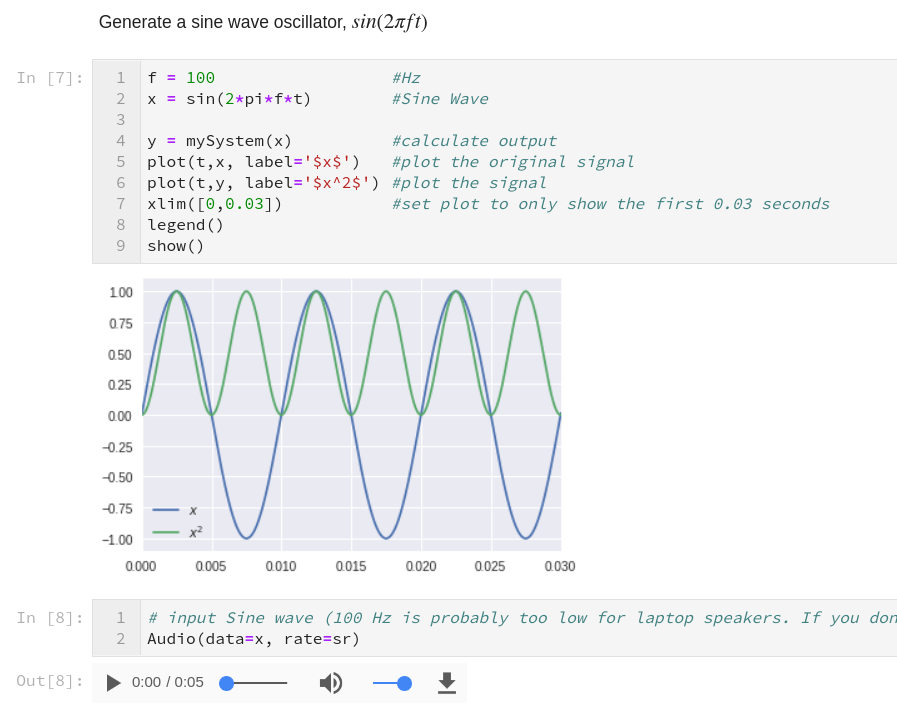
\includegraphics[width=\textwidth]{img/notenookExample.png}
	\caption[example of iPython notebook]
	{example of iPython notebook}
	\label{fig:ipython}
\end{figure}

\subsubsection*{GLSL}




\todo[inline]{unfinished}
In order to show examples in a highly common, industry standard video language, GLSL (Graphics Library Shading Language) code is provided. Examples can be run interactively on \link{http://shadertoy.com}{shadertoy.com}. Such examples will be highlighted with shadertoy's logo. Click the following to get to an example shader:\shader{https://www.shadertoy.com/view/ws3fD4}

\section{How to Describe Media Signals Mathematically}

If we want to talk about signals, or if we want to analyze them, it is often useful to look at the problem mathematically. First, let's introduce some conventions. They might look unfamiliar or complicated. But in fact it is not very complicated and knowing these conventions makes it easy to communicate (e.g. reading scientific papers about our topics or explaining something to another person).

\subsection*{Signals}
Mathematically speaking the types of signals we will be working with (images, audio, video, control signals) are \textit{functions}. The simplest of these cases is a mono audio signal. It is a function of time $t$, mapping a point in time to a value. If we call our signal $x$ we can write $x(t)$. A digital gray-scale image would complicate things since we would get one value only if we provide 2 coordinates. For example we could decide to call it $x$ and make it a function of horizontal and vertical coordinates, $u$ and $v$: $x(u,v)$. Maybe it is obvious that describing color video or multichannel audio starts to get a bit crowded\footnote{Take video for example. Video is a function of time and space(pixel coordinates). Color video has 3 to 4 channels. So, to retrieve a single value, we look at it as a function of time $t$, coordinates $u,v$ and channel number $c$: $x(t,u,v,c)$},so lets stick to mono audio for now.  

\begin{figure}[H]
	\centering
	% This file was created with tikzplotlib v0.9.14.
\begin{tikzpicture}

\definecolor{color0}{rgb}{0.12156862745098,0.466666666666667,0.705882352941177}

\begin{groupplot}[group style={group size=2 by 1}]
\nextgroupplot[
height=5cm,
legend cell align={left},
legend style={fill opacity=0.8, draw opacity=1, text opacity=1, draw=white!80!black},
tick align=outside,
tick pos=left,
width=7cm,
x grid style={white!69.0196078431373!black},
xlabel={\(\displaystyle t\), time[seconds]},
xmajorgrids,
xmin=-0.0483333333333333, xmax=1.015,
xtick style={color=black},
y grid style={white!69.0196078431373!black},
ylabel={\(\displaystyle y\)},
ymajorgrids,
ymin=0.0392144542339375, ymax=1.01832890308994,
ytick style={color=black}
]
\addplot [semithick, color0]
table {%
0 0.235621978151893
0.0333333333333333 0.973823700869215
0.0666666666666667 0.651665597627898
0.1 0.454633873381738
0.133333333333333 0.837279732850819
0.166666666666667 0.744984260241175
0.2 0.921901834079666
0.233333333333333 0.402807798332594
0.266666666666667 0.129684135121294
0.3 0.545110113821923
0.333333333333333 0.185968408195422
0.366666666666667 0.410019551441513
0.4 0.575660363580382
0.433333333333333 0.482259416743055
0.466666666666667 0.430973318905604
0.5 0.801034305349296
0.533333333333333 0.09294582932741
0.566666666666667 0.83892115766844
0.6 0.592937879796559
0.633333333333333 0.596004693829301
0.666666666666667 0.0837196564546649
0.7 0.578930005543894
0.733333333333333 0.673700691442343
0.766666666666667 0.198244046839318
0.8 0.516705292712326
0.833333333333333 0.140747087319865
0.866666666666667 0.43847563815737
0.9 0.696983632248657
0.933333333333333 0.328177900290687
0.966666666666667 0.159649425292901
};
\addlegendentry{$x(t)=y$}

\nextgroupplot[
height=5cm,
tick align=outside,
tick pos=left,
width=7cm,
x grid style={white!69.0196078431373!black},
xlabel={u},
xmin=-0.5, xmax=4.5,
xtick style={color=black},
y dir=reverse,
y grid style={white!69.0196078431373!black},
ylabel={v},
ymin=-0.5, ymax=4.5,
ytick style={color=black}
]
\addplot graphics [includegraphics cmd=\pgfimage,xmin=-0.5, xmax=4.5, ymin=4.5, ymax=-0.5] {plots/randSignal-000.png};
\end{groupplot}

\end{tikzpicture}

	% \includegraphics[width=11cm]{sineScatter}
	\caption[random signals]
	{two random signals. A one dimensional one, similar to mono audio and a two dimensional one, similar to a digital image.}
	\label{fig:randSigs}
\end{figure}



% Usually we describe a \textit{digital} signal by a name, say $x$, (but you can call it however you want). If we want to talk about the individual samples, or values of the (mono) signal, we can use a subscript or parenthesis. So if the fifth sample of $x$ is 1, we could write:

% \begin{equation}
% 	x_5=1
% \end{equation}
% or
% \begin{equation}
% 	x(5)=1
% \end{equation}
% Oftentimes we like to talk about a signal more generally and we use $n$ as a place holder for this index, so we might write $x_n$, meaning the nth sample of $x$.

\subsubsection*{Continuous Time vs Discrete Time}
In Figure \ref{fig:randSigs} we can see a plot if the function $x(t)$. Let's imagine for a moment that we have a simple sine wave as a function of time: $x(t) = sin(t)$. This function is defined for all values of $t$. It is \textit{continuous}. The same is true for $x(t) = t$ for example. But in this document, we concentrate on \textit{digital} signals. Digital signals are sampled at discrete points in time, so are not defined for all values of t. If we choose a sampling rate $f_s$ and therefore a sampling interval $t_s = \frac{1}{f_s}$. We create a new sampled \textit{discrete} function, $x_s(n)$ where n is any integer ($n \in \mathbb{Z}$). And we defined it so it is exactly the same as our original function $x$:
\begin{equation}
x_s(n) = x(n \cdot t_s)
\end{equation}

This idea is tried to visualize in Figure \ref{fig:sampledSine}. In this document we will sometimes treat signals as continuous time (defining signals as $x(t)$) and sometimes as discrete ($x(n)$). This is done to keep things as simple as possible. In the end, on a computer, signals are always discrete time signals.


\begin{figure}[h!]
	\centering
	% This file was created with tikzplotlib v0.9.14.
\begin{tikzpicture}

\definecolor{color0}{rgb}{0.12156862745098,0.466666666666667,0.705882352941177}

\begin{groupplot}[group style={group size=2 by 1}]
\nextgroupplot[
height=5cm,
legend cell align={left},
legend style={
  fill opacity=0.8,
  draw opacity=1,
  text opacity=1,
  at={(0.03,0.03)},
  anchor=south west,
  draw=white!80!black
},
tick align=outside,
tick pos=left,
width=8cm,
x grid style={white!69.0196078431373!black},
xlabel={\(\displaystyle t\), time[seconds]},
xmajorgrids,
xmin=-0.35, xmax=7.35,
xtick style={color=black},
y grid style={white!69.0196078431373!black},
ymajorgrids,
ymin=-1, ymax=1,
ytick style={color=black}
]
\addplot [semithick, color0]
table {%
0 0
0.0200573065902579 0.0200559617897853
0.0401146131805158 0.040103855425926
0.0601719197707736 0.0601356160004507
0.0802292263610315 0.0801431850954297
0.100286532951289 0.100118514024731
0.120343839541547 0.120053567071864
0.140401146131805 0.139940324722601
0.160458452722063 0.159770786891088
0.180515759312321 0.179536976138132
0.200573065902579 0.199230940880385
0.220630372492837 0.21884475858912
0.240687679083095 0.238370538977325
0.260744985673352 0.257800427173822
0.28080229226361 0.277126606883141
0.300859598853868 0.296341303529878
0.320916905444126 0.315436787386264
0.340974212034384 0.334405376681696
0.361031518624642 0.353239440692977
0.3810888252149 0.371931402814021
0.401146131805158 0.390473743603779
0.421203438395416 0.408859003811184
0.441260744985673 0.427079787375865
0.461318051575931 0.445128764403458
0.481375358166189 0.462998674114285
0.501432664756447 0.480682327764235
0.521489971346705 0.498172611536673
0.541547277936963 0.515462489404195
0.561604584527221 0.532545005959096
0.581661891117479 0.549413289211411
0.601719197707736 0.566060553353386
0.621776504297994 0.582480101489291
0.641833810888252 0.598665328329462
0.66189111747851 0.614609722847486
0.681948424068768 0.630306870899476
0.702005730659026 0.645750457804361
0.722063037249284 0.660934270884171
0.742120343839542 0.675852201963286
0.762177650429799 0.690498249825645
0.782234957020057 0.704866522628928
0.802292263610315 0.718951240274739
0.822349570200573 0.732746736733834
0.842406876790831 0.746247462325465
0.862464183381089 0.759447985949914
0.882521489971347 0.772342997273333
0.902578796561605 0.784927308863988
0.922636103151863 0.797195858279077
0.94269340974212 0.809143710101255
0.962750716332378 0.820766057924066
0.982808022922636 0.832058226285473
1.00286532951289 0.843015672548716
1.02292263610315 0.853633988729727
1.04297994269341 0.863908903270389
1.06303724928367 0.873836282756903
1.08309455587393 0.88341213358259
1.10315186246418 0.892632603554442
1.12320916905444 0.901493983442795
1.1432664756447 0.909992708473486
1.16332378223496 0.918125359761892
1.18338108882521 0.925888665688291
1.20343839541547 0.933279503213975
1.22349570200573 0.940294899137592
1.24355300859599 0.94693203129121
1.26361031518625 0.953188229675627
1.2836676217765 0.959060977534463
1.30372492836676 0.964547912366605
1.32378223495702 0.969646826876601
1.34383954154728 0.974355669862612
1.36389684813754 0.978672547041577
1.38395415472779 0.982595721811247
1.40401146131805 0.98612361594879
1.42406876790831 0.989254810245681
1.44412607449857 0.991988045078626
1.46418338108883 0.994322220916281
1.48424068767908 0.996256398761581
1.50429799426934 0.997789800529475
1.5243553008596 0.99892180935994
1.54441260744986 0.999651969866131
1.56446991404011 0.999979988317573
1.58452722063037 0.999905732758329
1.60458452722063 0.999429233060077
1.62464183381089 0.998550680910099
1.64469914040115 0.997270429734165
1.6647564469914 0.995588994554355
1.68481375358166 0.993507051781879
1.70487106017192 0.991025438944967
1.72492836676218 0.988145154351946
1.74498567335244 0.984867356689638
1.76504297994269 0.981193364557241
1.78510028653295 0.977124655935885
1.80515759312321 0.972662867594057
1.82521489971347 0.967809794429169
1.84527220630373 0.962567388745496
1.86532951289398 0.9569377594688
1.88538681948424 0.95092317129795
1.9054441260745 0.944526043793871
1.92550143266476 0.937748950406201
1.94555873925501 0.930594617438035
1.96561604584527 0.923065922949186
1.98567335243553 0.915165895598387
2.00573065902579 0.906897713424926
2.02578796561605 0.898264702570167
2.0458452722063 0.889270335939509
2.06590257879656 0.879918231805299
2.08595988538682 0.870212152351263
2.10601719197708 0.860156002159048
2.12607449856734 0.849753826637479
2.14613180515759 0.839009810395165
2.16618911174785 0.827928275557102
2.18624641833811 0.816513680025966
2.20630372492837 0.804770615688771
2.22636103151862 0.792703806569643
2.24641833810888 0.780318106929424
2.26647564469914 0.767618499312892
2.2865329512894 0.754610092544373
2.30659025787966 0.741298119672554
2.32664756446991 0.727687935865317
2.34670487106017 0.713785016255455
2.36676217765043 0.699594953738123
2.38681948424069 0.685123456720918
2.40687679083095 0.670376346827484
2.4269340974212 0.655359556555585
2.44699140401146 0.64007912689056
2.46704871060172 0.624541204875149
2.48710601719198 0.608752041136644
2.50716332378224 0.592717987372376
2.52722063037249 0.57644549379454
2.54727793696275 0.559941106535391
2.56733524355301 0.54321146501385
2.58739255014327 0.526263299264589
2.60744985673352 0.509103427230658
2.62750716332378 0.491738752020743
2.64756446991404 0.474176259132179
2.6676217765043 0.456423013640801
2.68767908309456 0.438486157358795
2.70773638968481 0.420372905961675
2.72779369627507 0.402090546085544
2.74785100286533 0.383646432395815
2.76790830945559 0.365047984628555
2.78796561604585 0.346302684605665
2.8080229226361 0.327418073225073
2.82808022922636 0.308401747427165
2.84813753581662 0.289261357138679
2.86819484240688 0.270004602195267
2.88825214899714 0.250639229243997
2.90830945558739 0.231173028627013
2.92836676217765 0.211613831247618
2.94842406876791 0.191969505420047
2.96848137535817 0.172247953704182
2.98853868194842 0.152457109726492
3.00859598853868 0.132604934988484
3.02865329512894 0.112699415663925
3.0487106017192 0.0927485593861576
3.06876790830946 0.0727603920267622
3.08882521489971 0.0527429544669016
3.10888252148997 0.0327042993626129
3.12893982808023 0.0126524879053722
3.14899713467049 -0.00740441342077986
3.16905444126075 -0.0274583360842407
3.189111747851 -0.0475012127516687
3.20916905444126 -0.0675249805333302
3.22922636103152 -0.0875215842266518
3.24928366762178 -0.107482979556686
3.26934097421203 -0.127401136412179
3.28939828080229 -0.147268042075939
3.30945558739255 -0.167075704448209
3.32951289398281 -0.186816155261746
3.34957020057307 -0.206481453287311
3.36962750716332 -0.226063687528284
3.38968481375358 -0.245554980403114
3.40974212034384 -0.264947490914332
3.4297994269341 -0.284233417802841
3.44985673352436 -0.303405002686224
3.46991404011461 -0.3224545331798
3.48997134670487 -0.34137434599918
3.51002865329513 -0.36015683004307
3.53008595988539 -0.378794429455077
3.55014326647564 -0.397279646663298
3.5702005730659 -0.415605045396454
3.59025787965616 -0.433763253675375
3.61031518624642 -0.45174696677861
3.63037249283668 -0.469548950180985
3.65042979942693 -0.487162042463929
3.67048710601719 -0.504579158196376
3.69054441260745 -0.521793290785112
3.71060171919771 -0.538797515293401
3.73065902578797 -0.555584991226761
3.75071633237822 -0.572148965284775
3.77077363896848 -0.588482774077819
3.79083094555874 -0.604579846807627
3.810888252149 -0.620433707910607
3.83094555873926 -0.636037979662837
3.85100286532951 -0.651386384745716
3.87106017191977 -0.666472748771215
3.89111747851003 -0.68129100276572
3.91117478510029 -0.695835185611472
3.93123209169054 -0.710099446444621
3.9512893982808 -0.72407804700892
3.97134670487106 -0.737765363964124
3.99140401146132 -0.751155891148157
4.01146131805158 -0.764244241792146
4.03151862464183 -0.777025150687419
4.05157593123209 -0.789493476303603
4.07163323782235 -0.801644202856972
4.09169054441261 -0.813472442328205
4.11174785100287 -0.824973436428749
4.13180515759312 -0.836142558514993
4.15186246418338 -0.846975315449485
4.17191977077364 -0.857467349408439
4.1919770773639 -0.867614439634809
4.21203438395415 -0.877412504136226
4.23209169054441 -0.886857601327107
4.25214899713467 -0.895945931614289
4.27220630372493 -0.904673838925531
4.29226361031519 -0.913037812180293
4.31232091690544 -0.921034486702175
4.3323782234957 -0.928660645572469
4.35243553008596 -0.935913220924267
4.37249283667622 -0.942789295176609
4.39255014326648 -0.949286102208173
4.41260744985673 -0.955401028470035
4.43266475644699 -0.961131614037057
4.45272206303725 -0.966475553597466
4.47277936962751 -0.97143069738024
4.49283667621776 -0.975995052019927
4.51289398280802 -0.980166781358535
4.53295128939828 -0.983944207184187
4.55300859598854 -0.987325809906237
4.5730659025788 -0.990310229166572
4.59312320916905 -0.992896264386862
4.61318051575931 -0.995082875251527
4.63323782234957 -0.996869182126243
4.65329512893983 -0.998254466411799
4.67335243553009 -0.999238170833177
4.69340974212034 -0.999819899663734
4.7134670487106 -0.999999418884399
4.73352435530086 -0.999776656277808
4.75358166189112 -0.999151701457363
4.77363896848138 -0.998124805831176
4.79369627507163 -0.996696382500937
4.81375358166189 -0.994867006095727
4.83381088825215 -0.992637412540857
4.85386819484241 -0.990008498761816
4.87392550143267 -0.986981322323459
4.89398280802292 -0.983557101004562
4.91404011461318 -0.979737212307935
4.93409742120344 -0.975523192906275
4.9541547277937 -0.970916738023992
4.97421203438395 -0.965919700755251
4.99426934097421 -0.960534091318504
5.01432664756447 -0.954762076247814
5.03438395415473 -0.948605977521299
5.05444126074499 -0.942068271627045
5.07449856733524 -0.935151588566852
5.0945558739255 -0.927858710798237
5.11461318051576 -0.920192572115099
5.13467048710602 -0.91215625646751
5.15472779369628 -0.903752996721089
5.17478510028653 -0.894986173356487
5.19484240687679 -0.885859313109477
5.21489971346705 -0.876376087552208
5.23495702005731 -0.866540311616204
5.25501432664757 -0.85635594205768
5.27507163323782 -0.845827075865811
5.29512893982808 -0.83495794861459
5.31518624641834 -0.823752932758929
5.3352435530086 -0.812216535875701
5.35530085959885 -0.80035339885042
5.37535816618911 -0.788168294010298
5.39541547277937 -0.775666123204427
5.41547277936963 -0.762851915831843
5.43553008595989 -0.749730826818299
5.45558739255014 -0.736308134542527
5.4756446991404 -0.722589238712841
5.49570200573066 -0.708579658194928
5.51575931232092 -0.694285028791714
5.53581661891118 -0.679711100976178
5.55587392550143 -0.664863737578038
5.57593123209169 -0.649748911425242
5.59598853868195 -0.634372702941208
5.61604584527221 -0.618741297698776
5.63610315186246 -0.602860983931862
5.65616045845272 -0.586738150005819
5.67621776504298 -0.570379281847508
5.69627507163324 -0.553790960336128
5.7163323782235 -0.536979858655846
5.73638968481375 -0.519952739611293
5.75644699140401 -0.502716452907013
5.77650429799427 -0.485277932391944
5.79656160458453 -0.467644193270063
5.81661891117479 -0.449822329278285
5.83667621776504 -0.431819509832789
5.8567335243553 -0.413642977144884
5.87679083094556 -0.395300043307605
5.89684813753582 -0.37679808735418
5.91690544412608 -0.358144552289583
5.93696275071633 -0.339346942096345
5.95702005730659 -0.320412818715837
5.97707736389685 -0.301349799006236
5.99713467048711 -0.282165551678401
6.01719197707736 -0.262867794210886
6.03724928366762 -0.243464289745338
6.05730659025788 -0.223962843963524
6.07736389684814 -0.204371301947247
6.0974212034384 -0.184697545022409
6.11747851002865 -0.164949487588491
6.13753581661891 -0.145135073934741
6.15759312320917 -0.125262275044322
6.17765042979943 -0.105339085387729
6.19770773638969 -0.0853735197067583
6.21776504297994 -0.0653736097903238
6.2378223495702 -0.045347401243406
6.25787965616046 -0.0253029502504529
6.27793696275072 -0.00524832033452392
6.29799426934097 0.0148084208865262
6.31805157593123 0.0348592049455024
6.33810888252149 0.0548959657716665
6.35816618911175 0.0749106429355779
6.37822349570201 0.0948951848916562
6.39828080229226 0.114841552217176
6.41833810888252 0.134741720846377
6.43839541547278 0.154587685298409
6.45845272206304 0.174371461897791
6.4785100286533 0.194085091986096
6.49856733524355 0.213720645123582
6.51862464183381 0.233270222279463
6.53868194842407 0.25272595900955
6.55873925501433 0.272080028619971
6.57879656160458 0.291324645315714
6.59885386819484 0.310452067332713
6.6189111747851 0.329454600052213
6.63896848137536 0.34832459909619
6.65902578796562 0.367054473402537
6.67908309455587 0.385636688278813
6.69914040114613 0.40406376843332
6.71919770773639 0.422328300982275
6.73925501432665 0.440422938431882
6.75931232091691 0.458340401634092
6.77936962750716 0.476073482714881
6.79942693409742 0.493615047973843
6.81948424068768 0.510958040753951
6.83954154727794 0.528095484280326
6.8595988538682 0.545020484466867
6.87965616045845 0.561726232689613
6.89971346704871 0.578206008525739
6.91977077363897 0.594453182457057
6.93982808022923 0.610461218536953
6.95988538681948 0.626223677019678
6.97994269340974 0.641734216950947
7 0.656986598718789
};
\addlegendentry{$x(t) = sin(t)$}

\nextgroupplot[
height=5cm,
legend cell align={left},
legend style={
  fill opacity=0.8,
  draw opacity=1,
  text opacity=1,
  at={(0.03,0.03)},
  anchor=south west,
  draw=white!80!black
},
tick align=outside,
tick pos=left,
width=8cm,
x grid style={white!69.0196078431373!black},
xlabel={\(\displaystyle n\), sample number/index},
xmajorgrids,
xmin=-1.7, xmax=35.7,
xtick style={color=black},
y grid style={white!69.0196078431373!black},
ymajorgrids,
ymin=-1, ymax=1,
ytick style={color=black}
]
\addplot [draw=color0, fill=color0, mark=*, only marks]
table{%
x  y
0 0
1 0.199230940880385
2 0.390473743603779
3 0.566060553353386
4 0.718951240274739
5 0.843015672548716
6 0.933279503213975
7 0.98612361594879
8 0.999429233060077
9 0.972662867594057
10 0.906897713424926
11 0.804770615688771
12 0.670376346827484
13 0.509103427230658
14 0.327418073225073
15 0.132604934988484
16 -0.0675249805333302
17 -0.264947490914332
18 -0.45174696677861
19 -0.620433707910607
20 -0.764244241792146
21 -0.877412504136226
22 -0.955401028470035
23 -0.995082875251527
24 -0.994867006095727
25 -0.954762076247814
26 -0.876376087552208
27 -0.762851915831843
28 -0.618741297698776
29 -0.449822329278285
30 -0.262867794210886
31 -0.0653736097903238
32 0.134741720846377
33 0.329454600052213
34 0.510958040753951
};
\addlegendentry{$x_s(n)=x(n\cdot t_s)=sin(n\cdot t_s)$}
\end{groupplot}

\end{tikzpicture}

	\caption[sampling]
	{A plot of a continuous variable, time $t$ and a discrete sampled ($t_s=0.2 seconds$) function of $n$.}
	\label{fig:sampledSine}
\end{figure}


\section{About plotting signals}

We will need to plot a lot of signals in order to understand them better. Most of the time, such a plot will look like figure \ref{fig:simpeSine}.

\begin{figure}[h!]
	\centering
	% This file was created with tikzplotlib v0.9.14.
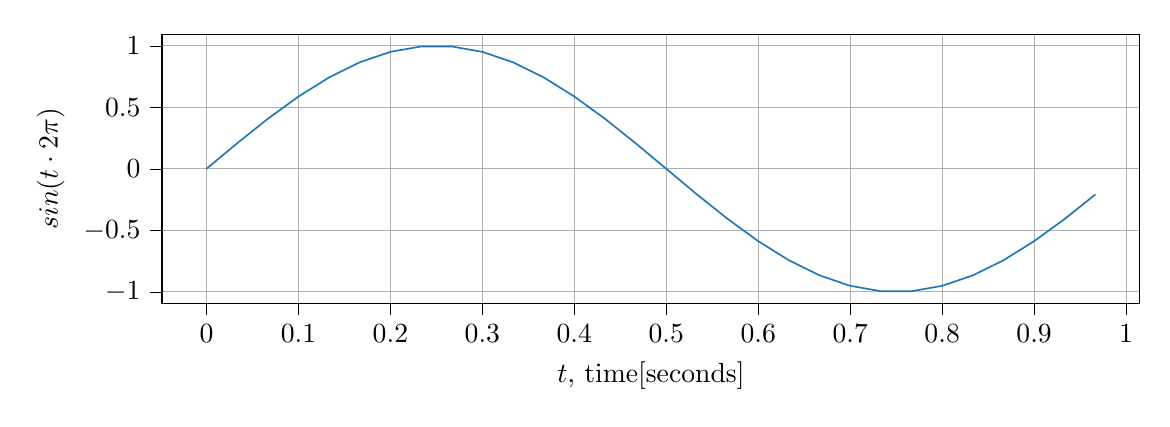
\begin{tikzpicture}

\definecolor{color0}{rgb}{0.12156862745098,0.466666666666667,0.705882352941177}

\begin{axis}[
height=5cm,
tick align=outside,
tick pos=left,
width=14cm,
x grid style={white!69.0196078431373!black},
xlabel={\(\displaystyle t\), time[seconds]},
xmajorgrids,
xmin=-0.0483333333333333, xmax=1.015,
xtick style={color=black},
y grid style={white!69.0196078431373!black},
ylabel={\(\displaystyle sin(t \cdot 2 \pi)\)},
ymajorgrids,
ymin=-1.0939740849051, ymax=1.0939740849051,
ytick style={color=black}
]
\addplot [semithick, color0]
table {%
0 0
0.0333333333333333 0.207911690817759
0.0666666666666667 0.4067366430758
0.1 0.587785252292473
0.133333333333333 0.743144825477394
0.166666666666667 0.866025403784439
0.2 0.951056516295154
0.233333333333333 0.994521895368273
0.266666666666667 0.994521895368273
0.3 0.951056516295154
0.333333333333333 0.866025403784439
0.366666666666667 0.743144825477394
0.4 0.587785252292473
0.433333333333333 0.4067366430758
0.466666666666667 0.207911690817759
0.5 1.22464679914735e-16
0.533333333333333 -0.207911690817759
0.566666666666667 -0.4067366430758
0.6 -0.587785252292473
0.633333333333333 -0.743144825477394
0.666666666666667 -0.866025403784438
0.7 -0.951056516295154
0.733333333333333 -0.994521895368273
0.766666666666667 -0.994521895368273
0.8 -0.951056516295154
0.833333333333333 -0.866025403784439
0.866666666666667 -0.743144825477394
0.9 -0.587785252292473
0.933333333333333 -0.4067366430758
0.966666666666667 -0.20791169081776
};
\end{axis}

\end{tikzpicture}

	% \includegraphics[width=11cm]{simpleSine}
	\caption[simple sine plot]
	{Sine wave, 1Hz, sampled at 30Hz sample rate}
	\label{fig:simpeSine}
\end{figure}

This plot looks nice but it has a problem. As just discussed, this sine wave is sampled at a sampling rate of 30 Hz, but we see a continuous line. This ``connection of the dots'' is created by plotting. It is kind of similar to what our \textit{digital-to-analog-converter} does. It somehow\footnote{linear interpolation in case of the plot} interpolates the values we have. \\
This can be misleading, so we should actually plot something more like figure \ref{fig:scatter}. Often we can see plots that look like figure \ref{fig:stem} as well when a signal is analyzed.

\begin{figure}[H]
	\centering
	% This file was created with tikzplotlib v0.9.14.
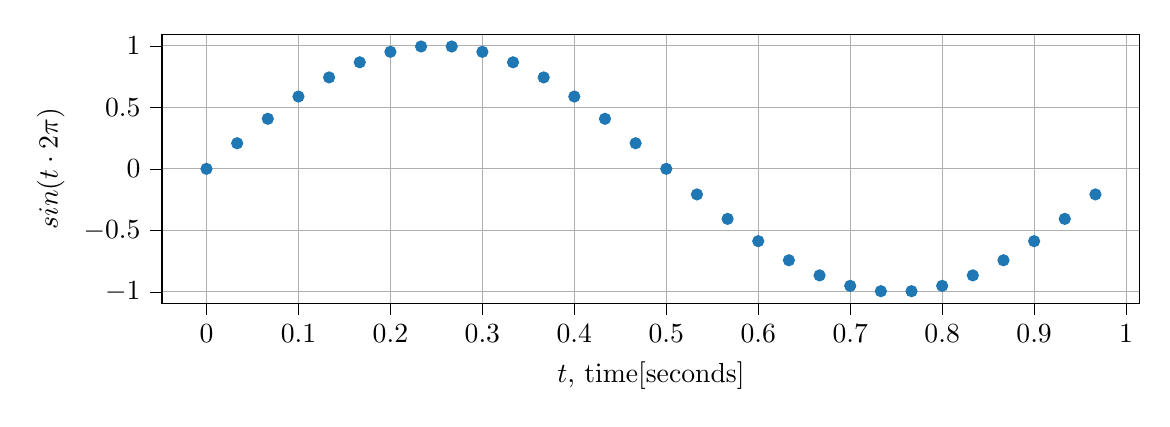
\begin{tikzpicture}

\definecolor{color0}{rgb}{0.12156862745098,0.466666666666667,0.705882352941177}

\begin{axis}[
height=5cm,
tick align=outside,
tick pos=left,
width=14cm,
x grid style={white!69.0196078431373!black},
xlabel={\(\displaystyle t\), time[seconds]},
xmajorgrids,
xmin=-0.0483333333333333, xmax=1.015,
xtick style={color=black},
y grid style={white!69.0196078431373!black},
ylabel={\(\displaystyle sin(t \cdot 2 \pi)\)},
ymajorgrids,
ymin=-1.0939740849051, ymax=1.0939740849051,
ytick style={color=black}
]
\addplot [draw=color0, fill=color0, mark=*, only marks]
table{%
x  y
0 0
0.0333333333333333 0.207911690817759
0.0666666666666667 0.4067366430758
0.1 0.587785252292473
0.133333333333333 0.743144825477394
0.166666666666667 0.866025403784439
0.2 0.951056516295154
0.233333333333333 0.994521895368273
0.266666666666667 0.994521895368273
0.3 0.951056516295154
0.333333333333333 0.866025403784439
0.366666666666667 0.743144825477394
0.4 0.587785252292473
0.433333333333333 0.4067366430758
0.466666666666667 0.207911690817759
0.5 1.22464679914735e-16
0.533333333333333 -0.207911690817759
0.566666666666667 -0.4067366430758
0.6 -0.587785252292473
0.633333333333333 -0.743144825477394
0.666666666666667 -0.866025403784438
0.7 -0.951056516295154
0.733333333333333 -0.994521895368273
0.766666666666667 -0.994521895368273
0.8 -0.951056516295154
0.833333333333333 -0.866025403784439
0.866666666666667 -0.743144825477394
0.9 -0.587785252292473
0.933333333333333 -0.4067366430758
0.966666666666667 -0.20791169081776
};
\end{axis}

\end{tikzpicture}

	% \includegraphics[width=11cm]{sineScatter}
	\caption[Sine scatter-plot]
	{Sine wave, 1Hz, sample rate 30Hz, scatter-plot}
	\label{fig:scatter}
\end{figure}



\begin{figure}[H]
	\centering
	% This file was created with tikzplotlib v0.9.14.
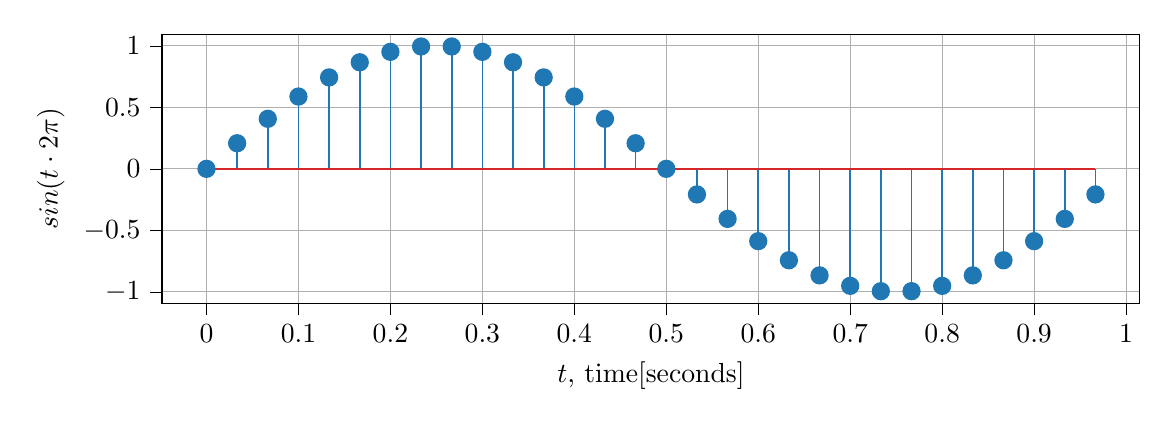
\begin{tikzpicture}

\definecolor{color0}{rgb}{0.12156862745098,0.466666666666667,0.705882352941177}
\definecolor{color1}{rgb}{0.83921568627451,0.152941176470588,0.156862745098039}

\begin{axis}[
height=5cm,
tick align=outside,
tick pos=left,
width=14cm,
x grid style={white!69.0196078431373!black},
xlabel={\(\displaystyle t\), time[seconds]},
xmajorgrids,
xmin=-0.0483333333333333, xmax=1.015,
xtick style={color=black},
y grid style={white!69.0196078431373!black},
ylabel={\(\displaystyle sin(t \cdot 2 \pi)\)},
ymajorgrids,
ymin=-1.0939740849051, ymax=1.0939740849051,
ytick style={color=black}
]
\addplot [semithick, color0]
table {%
0 0
0 0
};
\addplot [semithick, color0]
table {%
0.0333333333333333 0
0.0333333333333333 0.207911690817759
};
\addplot [semithick, color0]
table {%
0.0666666666666667 0
0.0666666666666667 0.4067366430758
};
\addplot [semithick, color0]
table {%
0.1 0
0.1 0.587785252292473
};
\addplot [semithick, color0]
table {%
0.133333333333333 0
0.133333333333333 0.743144825477394
};
\addplot [semithick, color0]
table {%
0.166666666666667 0
0.166666666666667 0.866025403784439
};
\addplot [semithick, color0]
table {%
0.2 0
0.2 0.951056516295154
};
\addplot [semithick, color0]
table {%
0.233333333333333 0
0.233333333333333 0.994521895368273
};
\addplot [semithick, color0]
table {%
0.266666666666667 0
0.266666666666667 0.994521895368273
};
\addplot [semithick, color0]
table {%
0.3 0
0.3 0.951056516295154
};
\addplot [semithick, color0]
table {%
0.333333333333333 0
0.333333333333333 0.866025403784439
};
\addplot [semithick, color0]
table {%
0.366666666666667 0
0.366666666666667 0.743144825477394
};
\addplot [semithick, color0]
table {%
0.4 0
0.4 0.587785252292473
};
\addplot [semithick, color0]
table {%
0.433333333333333 0
0.433333333333333 0.4067366430758
};
\addplot [semithick, color0]
table {%
0.466666666666667 0
0.466666666666667 0.207911690817759
};
\addplot [semithick, color0]
table {%
0.5 0
0.5 1.22464679914735e-16
};
\addplot [semithick, color0]
table {%
0.533333333333333 0
0.533333333333333 -0.207911690817759
};
\addplot [semithick, color0]
table {%
0.566666666666667 0
0.566666666666667 -0.4067366430758
};
\addplot [semithick, color0]
table {%
0.6 0
0.6 -0.587785252292473
};
\addplot [semithick, color0]
table {%
0.633333333333333 0
0.633333333333333 -0.743144825477394
};
\addplot [semithick, color0]
table {%
0.666666666666667 0
0.666666666666667 -0.866025403784438
};
\addplot [semithick, color0]
table {%
0.7 0
0.7 -0.951056516295154
};
\addplot [semithick, color0]
table {%
0.733333333333333 0
0.733333333333333 -0.994521895368273
};
\addplot [semithick, color0]
table {%
0.766666666666667 0
0.766666666666667 -0.994521895368273
};
\addplot [semithick, color0]
table {%
0.8 0
0.8 -0.951056516295154
};
\addplot [semithick, color0]
table {%
0.833333333333333 0
0.833333333333333 -0.866025403784439
};
\addplot [semithick, color0]
table {%
0.866666666666667 0
0.866666666666667 -0.743144825477394
};
\addplot [semithick, color0]
table {%
0.9 0
0.9 -0.587785252292473
};
\addplot [semithick, color0]
table {%
0.933333333333333 0
0.933333333333333 -0.4067366430758
};
\addplot [semithick, color0]
table {%
0.966666666666667 0
0.966666666666667 -0.20791169081776
};
\addplot [semithick, color0, mark=*, mark size=3, mark options={solid}, only marks]
table {%
0 0
0.0333333333333333 0.207911690817759
0.0666666666666667 0.4067366430758
0.1 0.587785252292473
0.133333333333333 0.743144825477394
0.166666666666667 0.866025403784439
0.2 0.951056516295154
0.233333333333333 0.994521895368273
0.266666666666667 0.994521895368273
0.3 0.951056516295154
0.333333333333333 0.866025403784439
0.366666666666667 0.743144825477394
0.4 0.587785252292473
0.433333333333333 0.4067366430758
0.466666666666667 0.207911690817759
0.5 1.22464679914735e-16
0.533333333333333 -0.207911690817759
0.566666666666667 -0.4067366430758
0.6 -0.587785252292473
0.633333333333333 -0.743144825477394
0.666666666666667 -0.866025403784438
0.7 -0.951056516295154
0.733333333333333 -0.994521895368273
0.766666666666667 -0.994521895368273
0.8 -0.951056516295154
0.833333333333333 -0.866025403784439
0.866666666666667 -0.743144825477394
0.9 -0.587785252292473
0.933333333333333 -0.4067366430758
0.966666666666667 -0.20791169081776
};
\addplot [semithick, color1]
table {%
0 0
0.966666666666667 0
};
\end{axis}

\end{tikzpicture}

	% \includegraphics[width=11cm]{sineStem}
	\caption[sine stem plot]
	{Sine wave, 1Hz, sample rate 30Hz, stem-plot}
	\label{fig:stem}
\end{figure}


So why don't we always do a stem- or scatter-plot? Simply because it gets too crowded with our usual sampling rates in audio. It just works with very low sampling rates or very short signals.\\
\begin{figure}[H]
	\centering
	\includegraphics[width=11cm]{stem44100}
	\caption[sine stem plot, crowded]
	{Sine wave, 1Hz, sample rate 44100Hz, stem-plot}
	\label{fig:sine1HzStemPlot}
\end{figure}
\textbf{But we should never forget that we don't actually have the values in between the dots. Digital signals are not defined between their sampled points.}

You can look at how these signals where generated and plotted in this Notebook:\colab{https://colab.research.google.com/github/hrtlacek/dspCourse/blob/master/notebooks/00\_Introduction.ipynb}
 % \link{https://colab.research.google.com/github/hrtlacek/dspCourse/blob/master/notebooks/00\_Introduction.ipynb}{in this Notebook}

\subsection{Looking at Signals in Max}
\todo[inline]{todo}
\begin{figure}[H]
	\centering
	% % This file was created with tikzplotlib v0.9.14.
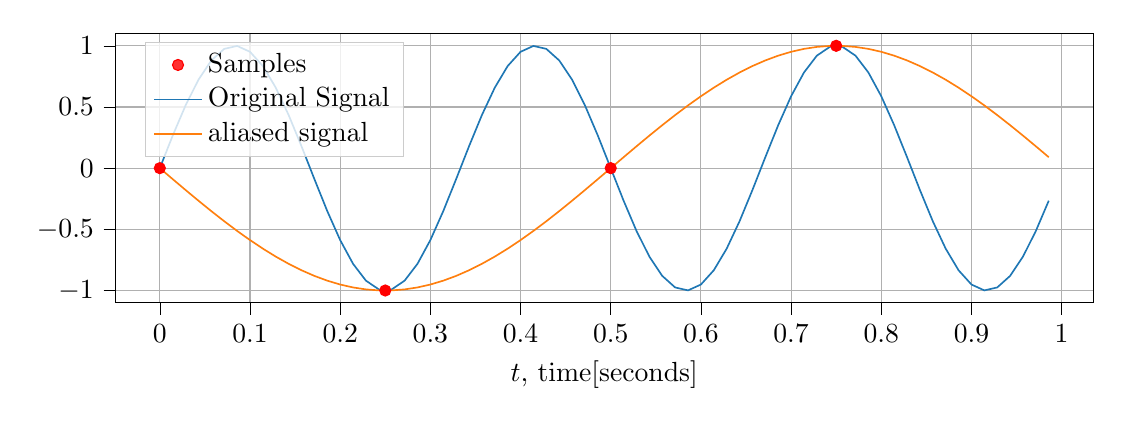
\begin{tikzpicture}

\definecolor{color0}{rgb}{0.12156862745098,0.466666666666667,0.705882352941177}
\definecolor{color1}{rgb}{1,0.498039215686275,0.0549019607843137}

\begin{axis}[
height=5cm,
legend cell align={left},
legend style={
  fill opacity=0.8,
  draw opacity=1,
  text opacity=1,
  at={(0.03,0.97)},
  anchor=north west,
  draw=white!80!black
},
tick align=outside,
tick pos=left,
width=14cm,
x grid style={white!69.0196078431373!black},
xlabel={\(\displaystyle t\), time[seconds]},
xmajorgrids,
xmin=-0.0492857142857143, xmax=1.035,
xtick style={color=black},
y grid style={white!69.0196078431373!black},
ymajorgrids,
ymin=-1.1, ymax=1.1,
ytick style={color=black}
]
\addplot [draw=red, fill=red, mark=*, only marks]
table{%
x  y
0 0
0.25 -1
0.5 3.67394039744206e-16
0.75 1
};
\addlegendentry{Samples}
\addplot [semithick, color0]
table {%
0 0
0.0142857142857143 0.266036845566675
0.0285714285714286 0.512899277405906
0.0428571428571429 0.722794863827392
0.0571428571428571 0.880595531856738
0.0714285714285714 0.974927912181824
0.0857142857142857 0.998993066541315
0.1 0.951056516295154
0.114285714285714 0.834573253721303
0.128571428571429 0.657938725939713
0.142857142857143 0.433883739117558
0.157142857142857 0.178556894798637
0.171428571428571 -0.0896393089034334
0.185714285714286 -0.351374824081343
0.2 -0.587785252292473
0.214285714285714 -0.78183148246803
0.228571428571429 -0.919527772551451
0.242857142857143 -0.990949761767935
0.257142857142857 -0.990949761767935
0.271428571428571 -0.919527772551451
0.285714285714286 -0.78183148246803
0.3 -0.587785252292473
0.314285714285714 -0.351374824081343
0.328571428571429 -0.0896393089034337
0.342857142857143 0.178556894798636
0.357142857142857 0.433883739117558
0.371428571428571 0.657938725939712
0.385714285714286 0.834573253721303
0.4 0.951056516295154
0.414285714285714 0.998993066541315
0.428571428571429 0.974927912181824
0.442857142857143 0.880595531856738
0.457142857142857 0.722794863827392
0.471428571428571 0.512899277405906
0.485714285714286 0.266036845566675
0.5 3.67394039744206e-16
0.514285714285714 -0.266036845566673
0.528571428571429 -0.512899277405906
0.542857142857143 -0.72279486382739
0.557142857142857 -0.880595531856738
0.571428571428571 -0.974927912181824
0.585714285714286 -0.998993066541315
0.6 -0.951056516295154
0.614285714285714 -0.834573253721302
0.628571428571429 -0.657938725939713
0.642857142857143 -0.433883739117559
0.657142857142857 -0.178556894798637
0.671428571428571 0.089639308903433
0.685714285714286 0.351374824081342
0.7 0.587785252292473
0.714285714285714 0.781831482468029
0.728571428571429 0.91952777255145
0.742857142857143 0.990949761767935
0.757142857142857 0.990949761767935
0.771428571428571 0.919527772551451
0.785714285714286 0.78183148246803
0.8 0.587785252292474
0.814285714285714 0.351374824081343
0.828571428571429 0.0896393089034341
0.842857142857143 -0.178556894798636
0.857142857142857 -0.433883739117558
0.871428571428571 -0.657938725939712
0.885714285714286 -0.834573253721302
0.9 -0.951056516295153
0.914285714285714 -0.998993066541315
0.928571428571429 -0.974927912181824
0.942857142857143 -0.880595531856738
0.957142857142857 -0.722794863827392
0.971428571428571 -0.512899277405907
0.985714285714286 -0.266036845566676
};
\addlegendentry{Original Signal}
\addplot [semithick, color1]
table {%
0 -0
0.0142857142857143 -0.0896393089034335
0.0285714285714286 -0.178556894798637
0.0428571428571429 -0.266036845566675
0.0571428571428571 -0.351374824081343
0.0714285714285714 -0.433883739117558
0.0857142857142857 -0.512899277405906
0.1 -0.587785252292473
0.114285714285714 -0.657938725939713
0.128571428571429 -0.722794863827391
0.142857142857143 -0.78183148246803
0.157142857142857 -0.834573253721303
0.171428571428571 -0.880595531856738
0.185714285714286 -0.919527772551451
0.2 -0.951056516295154
0.214285714285714 -0.974927912181824
0.228571428571429 -0.990949761767935
0.242857142857143 -0.998993066541315
0.257142857142857 -0.998993066541315
0.271428571428571 -0.990949761767935
0.285714285714286 -0.974927912181824
0.3 -0.951056516295154
0.314285714285714 -0.919527772551451
0.328571428571429 -0.880595531856738
0.342857142857143 -0.834573253721303
0.357142857142857 -0.78183148246803
0.371428571428571 -0.722794863827392
0.385714285714286 -0.657938725939713
0.4 -0.587785252292473
0.414285714285714 -0.512899277405906
0.428571428571429 -0.433883739117558
0.442857142857143 -0.351374824081343
0.457142857142857 -0.266036845566675
0.471428571428571 -0.178556894798637
0.485714285714286 -0.0896393089034336
0.5 -1.22464679914735e-16
0.514285714285714 0.0896393089034329
0.528571428571429 0.178556894798637
0.542857142857143 0.266036845566675
0.557142857142857 0.351374824081343
0.571428571428571 0.433883739117558
0.585714285714286 0.512899277405906
0.6 0.587785252292473
0.614285714285714 0.657938725939713
0.628571428571429 0.722794863827391
0.642857142857143 0.78183148246803
0.657142857142857 0.834573253721303
0.671428571428571 0.880595531856738
0.685714285714286 0.919527772551451
0.7 0.951056516295154
0.714285714285714 0.974927912181824
0.728571428571429 0.990949761767935
0.742857142857143 0.998993066541315
0.757142857142857 0.998993066541315
0.771428571428571 0.990949761767935
0.785714285714286 0.974927912181824
0.8 0.951056516295154
0.814285714285714 0.919527772551451
0.828571428571429 0.880595531856738
0.842857142857143 0.834573253721303
0.857142857142857 0.78183148246803
0.871428571428571 0.722794863827392
0.885714285714286 0.657938725939713
0.9 0.587785252292473
0.914285714285714 0.512899277405906
0.928571428571429 0.433883739117558
0.942857142857143 0.351374824081343
0.957142857142857 0.266036845566675
0.971428571428571 0.178556894798637
0.985714285714286 0.0896393089034337
};
\addlegendentry{aliased signal}
\end{axis}

\end{tikzpicture}

	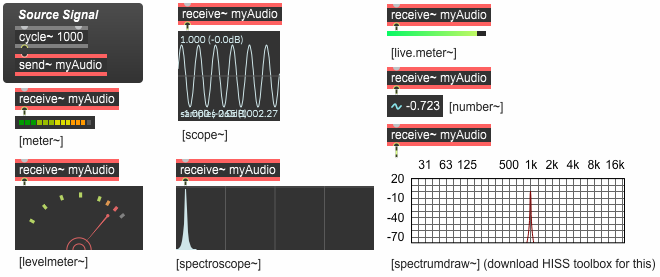
\includegraphics{metering}
	\caption[metering]
	{Metering Audio in Max}
	\label{fig:meteringAudio}
\end{figure}


\begin{figure}[H]
	\centering
	% % This file was created with tikzplotlib v0.9.14.
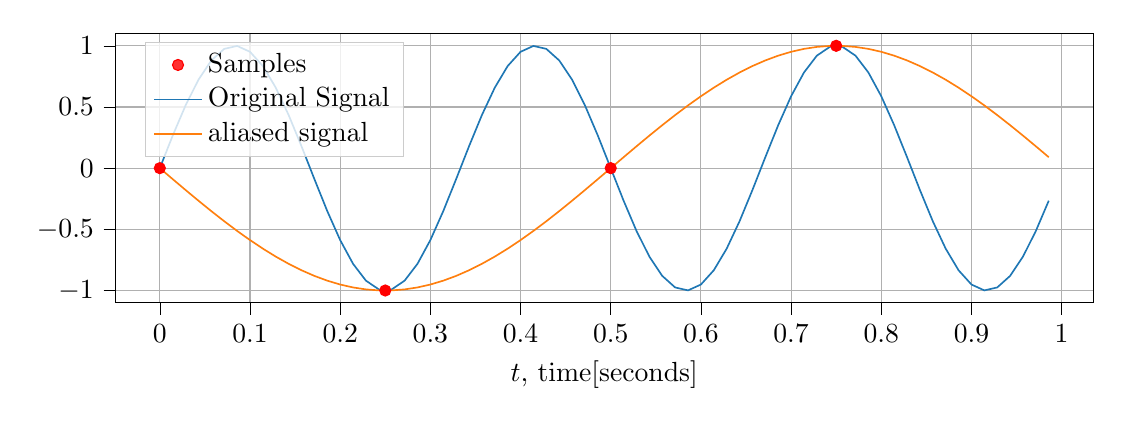
\begin{tikzpicture}

\definecolor{color0}{rgb}{0.12156862745098,0.466666666666667,0.705882352941177}
\definecolor{color1}{rgb}{1,0.498039215686275,0.0549019607843137}

\begin{axis}[
height=5cm,
legend cell align={left},
legend style={
  fill opacity=0.8,
  draw opacity=1,
  text opacity=1,
  at={(0.03,0.97)},
  anchor=north west,
  draw=white!80!black
},
tick align=outside,
tick pos=left,
width=14cm,
x grid style={white!69.0196078431373!black},
xlabel={\(\displaystyle t\), time[seconds]},
xmajorgrids,
xmin=-0.0492857142857143, xmax=1.035,
xtick style={color=black},
y grid style={white!69.0196078431373!black},
ymajorgrids,
ymin=-1.1, ymax=1.1,
ytick style={color=black}
]
\addplot [draw=red, fill=red, mark=*, only marks]
table{%
x  y
0 0
0.25 -1
0.5 3.67394039744206e-16
0.75 1
};
\addlegendentry{Samples}
\addplot [semithick, color0]
table {%
0 0
0.0142857142857143 0.266036845566675
0.0285714285714286 0.512899277405906
0.0428571428571429 0.722794863827392
0.0571428571428571 0.880595531856738
0.0714285714285714 0.974927912181824
0.0857142857142857 0.998993066541315
0.1 0.951056516295154
0.114285714285714 0.834573253721303
0.128571428571429 0.657938725939713
0.142857142857143 0.433883739117558
0.157142857142857 0.178556894798637
0.171428571428571 -0.0896393089034334
0.185714285714286 -0.351374824081343
0.2 -0.587785252292473
0.214285714285714 -0.78183148246803
0.228571428571429 -0.919527772551451
0.242857142857143 -0.990949761767935
0.257142857142857 -0.990949761767935
0.271428571428571 -0.919527772551451
0.285714285714286 -0.78183148246803
0.3 -0.587785252292473
0.314285714285714 -0.351374824081343
0.328571428571429 -0.0896393089034337
0.342857142857143 0.178556894798636
0.357142857142857 0.433883739117558
0.371428571428571 0.657938725939712
0.385714285714286 0.834573253721303
0.4 0.951056516295154
0.414285714285714 0.998993066541315
0.428571428571429 0.974927912181824
0.442857142857143 0.880595531856738
0.457142857142857 0.722794863827392
0.471428571428571 0.512899277405906
0.485714285714286 0.266036845566675
0.5 3.67394039744206e-16
0.514285714285714 -0.266036845566673
0.528571428571429 -0.512899277405906
0.542857142857143 -0.72279486382739
0.557142857142857 -0.880595531856738
0.571428571428571 -0.974927912181824
0.585714285714286 -0.998993066541315
0.6 -0.951056516295154
0.614285714285714 -0.834573253721302
0.628571428571429 -0.657938725939713
0.642857142857143 -0.433883739117559
0.657142857142857 -0.178556894798637
0.671428571428571 0.089639308903433
0.685714285714286 0.351374824081342
0.7 0.587785252292473
0.714285714285714 0.781831482468029
0.728571428571429 0.91952777255145
0.742857142857143 0.990949761767935
0.757142857142857 0.990949761767935
0.771428571428571 0.919527772551451
0.785714285714286 0.78183148246803
0.8 0.587785252292474
0.814285714285714 0.351374824081343
0.828571428571429 0.0896393089034341
0.842857142857143 -0.178556894798636
0.857142857142857 -0.433883739117558
0.871428571428571 -0.657938725939712
0.885714285714286 -0.834573253721302
0.9 -0.951056516295153
0.914285714285714 -0.998993066541315
0.928571428571429 -0.974927912181824
0.942857142857143 -0.880595531856738
0.957142857142857 -0.722794863827392
0.971428571428571 -0.512899277405907
0.985714285714286 -0.266036845566676
};
\addlegendentry{Original Signal}
\addplot [semithick, color1]
table {%
0 -0
0.0142857142857143 -0.0896393089034335
0.0285714285714286 -0.178556894798637
0.0428571428571429 -0.266036845566675
0.0571428571428571 -0.351374824081343
0.0714285714285714 -0.433883739117558
0.0857142857142857 -0.512899277405906
0.1 -0.587785252292473
0.114285714285714 -0.657938725939713
0.128571428571429 -0.722794863827391
0.142857142857143 -0.78183148246803
0.157142857142857 -0.834573253721303
0.171428571428571 -0.880595531856738
0.185714285714286 -0.919527772551451
0.2 -0.951056516295154
0.214285714285714 -0.974927912181824
0.228571428571429 -0.990949761767935
0.242857142857143 -0.998993066541315
0.257142857142857 -0.998993066541315
0.271428571428571 -0.990949761767935
0.285714285714286 -0.974927912181824
0.3 -0.951056516295154
0.314285714285714 -0.919527772551451
0.328571428571429 -0.880595531856738
0.342857142857143 -0.834573253721303
0.357142857142857 -0.78183148246803
0.371428571428571 -0.722794863827392
0.385714285714286 -0.657938725939713
0.4 -0.587785252292473
0.414285714285714 -0.512899277405906
0.428571428571429 -0.433883739117558
0.442857142857143 -0.351374824081343
0.457142857142857 -0.266036845566675
0.471428571428571 -0.178556894798637
0.485714285714286 -0.0896393089034336
0.5 -1.22464679914735e-16
0.514285714285714 0.0896393089034329
0.528571428571429 0.178556894798637
0.542857142857143 0.266036845566675
0.557142857142857 0.351374824081343
0.571428571428571 0.433883739117558
0.585714285714286 0.512899277405906
0.6 0.587785252292473
0.614285714285714 0.657938725939713
0.628571428571429 0.722794863827391
0.642857142857143 0.78183148246803
0.657142857142857 0.834573253721303
0.671428571428571 0.880595531856738
0.685714285714286 0.919527772551451
0.7 0.951056516295154
0.714285714285714 0.974927912181824
0.728571428571429 0.990949761767935
0.742857142857143 0.998993066541315
0.757142857142857 0.998993066541315
0.771428571428571 0.990949761767935
0.785714285714286 0.974927912181824
0.8 0.951056516295154
0.814285714285714 0.919527772551451
0.828571428571429 0.880595531856738
0.842857142857143 0.834573253721303
0.857142857142857 0.78183148246803
0.871428571428571 0.722794863827392
0.885714285714286 0.657938725939713
0.9 0.587785252292473
0.914285714285714 0.512899277405906
0.928571428571429 0.433883739117558
0.942857142857143 0.351374824081343
0.957142857142857 0.266036845566675
0.971428571428571 0.178556894798637
0.985714285714286 0.0896393089034337
};
\addlegendentry{aliased signal}
\end{axis}

\end{tikzpicture}

	\includegraphics[width = \textwidth]{img/lookAtMatrix.png}
	\caption[metering]
	{Inspecting Jitter Matrices in Max}
	\label{fig:matrixIns[ection]}
\end{figure}



\section{What is aliasing?}
Aliasing in audio means problems caused by signals that exceed the nyquist rate.\\
The nyquist rate, let's call it $f_n$ for now, is defined by the half of the sample rate ($f_s$). So,
\begin{equation}
	f_n=\frac{f_s}{2}
\end{equation}
A digital system can only describe signals up to its nyquist rate. If we try to make signals higher than this frequency, we will fail and encounter strange effects. So the idea is that the highest frequency in a signal $f_{max}$ should be lower than half the sampling rate. This is called the \textit{Nyquist criterion}:\\
\begin{equation}
f_{max} < \frac{f_s}{2} 
\end{equation}
This is the same as saying the sampling rate should be at least double the highest frequency in the signal of interest:
\begin{equation}
f_{max}\cdot2 < f_s 
\end{equation}

Visually speaking, frequencies higher than nyquist fold back. So, let's assume we have a sampling rate of 100Hz. Nyquist would be at 50Hz. If we try to synthesize a sine wave with 51Hz, what we will get is a 49Hz one. If we try to make a 52Hz one, we will get 48Hz. So you see, it simply folds back. You can find an interactive example \link{https://jackschaedler.github.io/circles-sines-signals/sampling.html}{here}.

\begin{framed}
	\textbf{Video analogies}\\
	Aliasing in graphics usually means \textit{spacial} aliasing, so aliasing in the space domain. This is what we see in figure \ref{fig:spAlias}. But there is also time domain aliasing in film. It is actually more natural to think about the sampling rate in audio as the same as the frame rate in video. For some really weird effects that arise in video due to time domain aliasing see \href{https://www.youtube.com/watch?v=LVwmtwZLG88}{airplane}\footnotemark , \href{https://www.youtube.com/watch?v=GBtHeR-hY9Y}{Water experiment}\footnotemark or \href{https://www.youtube.com/watch?v=jcOKTTnOIV8}{Guitar strings}\footnotemark .
	The \textit{moiré pattern} is also an example of aliasing. Figures \ref{fig:moire1} and \ref{fig:moire2} are stills generated with a shader you can find here: \shader{https://www.shadertoy.com/view/NdKSDz}. It essentially renders a varying amount of circles, resulting in aliasing. 

	\begin{center}
		% \centering
		
\includegraphics[width=7cm]{moire1.png}
		\captionof{figure}{A couple of circles without moiré pattern.}
		\label{fig:moire1}
	\end{center}
	\begin{center}
		% \centering
		
\includegraphics[width=7cm]{moire2.png}
		\captionof{figure}{Much more circles, resulting in a moiré pattern.}
		\label{fig:moire2}
	\end{center}

	\begin{center}
		% \centering
		\includegraphics[width=7cm]{spacialAliasing1.png}
		\captionof{figure}{Spacial aliasing in graphics. The ``frequency'' of the intended pixels is to high for the actual pixels.}
		\label{fig:spAlias}
	\end{center}
	The particularly strange effects in the airplane example above are caused by the rolling shutter of a CMOS sensor. Since it is not sampling the incoming light uniformly (at the same time) the image is distorted.
\end{framed}
\footnotetext[2]{https://www.youtube.com/watch?v=LVwmtwZLG88}
\footnotetext[3]{https://www.youtube.com/watch?v=GBtHeR-hY9Y}
\footnotetext[4]{https://www.youtube.com/watch?v=jcOKTTnOIV8}


In figure \ref{fig:cosAlias} you can see a visualization of aliasing in the time domain.

\begin{figure}[H]
	\centering
	% This file was created with tikzplotlib v0.9.14.
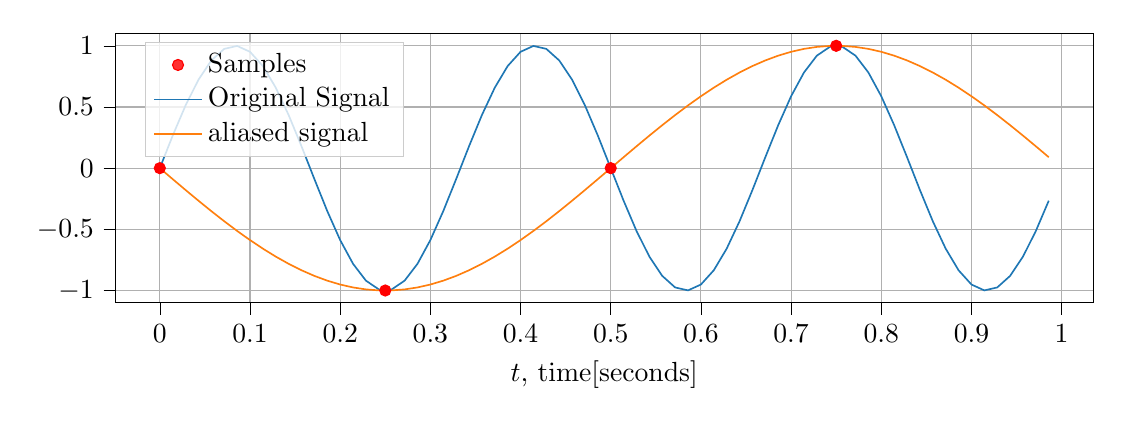
\begin{tikzpicture}

\definecolor{color0}{rgb}{0.12156862745098,0.466666666666667,0.705882352941177}
\definecolor{color1}{rgb}{1,0.498039215686275,0.0549019607843137}

\begin{axis}[
height=5cm,
legend cell align={left},
legend style={
  fill opacity=0.8,
  draw opacity=1,
  text opacity=1,
  at={(0.03,0.97)},
  anchor=north west,
  draw=white!80!black
},
tick align=outside,
tick pos=left,
width=14cm,
x grid style={white!69.0196078431373!black},
xlabel={\(\displaystyle t\), time[seconds]},
xmajorgrids,
xmin=-0.0492857142857143, xmax=1.035,
xtick style={color=black},
y grid style={white!69.0196078431373!black},
ymajorgrids,
ymin=-1.1, ymax=1.1,
ytick style={color=black}
]
\addplot [draw=red, fill=red, mark=*, only marks]
table{%
x  y
0 0
0.25 -1
0.5 3.67394039744206e-16
0.75 1
};
\addlegendentry{Samples}
\addplot [semithick, color0]
table {%
0 0
0.0142857142857143 0.266036845566675
0.0285714285714286 0.512899277405906
0.0428571428571429 0.722794863827392
0.0571428571428571 0.880595531856738
0.0714285714285714 0.974927912181824
0.0857142857142857 0.998993066541315
0.1 0.951056516295154
0.114285714285714 0.834573253721303
0.128571428571429 0.657938725939713
0.142857142857143 0.433883739117558
0.157142857142857 0.178556894798637
0.171428571428571 -0.0896393089034334
0.185714285714286 -0.351374824081343
0.2 -0.587785252292473
0.214285714285714 -0.78183148246803
0.228571428571429 -0.919527772551451
0.242857142857143 -0.990949761767935
0.257142857142857 -0.990949761767935
0.271428571428571 -0.919527772551451
0.285714285714286 -0.78183148246803
0.3 -0.587785252292473
0.314285714285714 -0.351374824081343
0.328571428571429 -0.0896393089034337
0.342857142857143 0.178556894798636
0.357142857142857 0.433883739117558
0.371428571428571 0.657938725939712
0.385714285714286 0.834573253721303
0.4 0.951056516295154
0.414285714285714 0.998993066541315
0.428571428571429 0.974927912181824
0.442857142857143 0.880595531856738
0.457142857142857 0.722794863827392
0.471428571428571 0.512899277405906
0.485714285714286 0.266036845566675
0.5 3.67394039744206e-16
0.514285714285714 -0.266036845566673
0.528571428571429 -0.512899277405906
0.542857142857143 -0.72279486382739
0.557142857142857 -0.880595531856738
0.571428571428571 -0.974927912181824
0.585714285714286 -0.998993066541315
0.6 -0.951056516295154
0.614285714285714 -0.834573253721302
0.628571428571429 -0.657938725939713
0.642857142857143 -0.433883739117559
0.657142857142857 -0.178556894798637
0.671428571428571 0.089639308903433
0.685714285714286 0.351374824081342
0.7 0.587785252292473
0.714285714285714 0.781831482468029
0.728571428571429 0.91952777255145
0.742857142857143 0.990949761767935
0.757142857142857 0.990949761767935
0.771428571428571 0.919527772551451
0.785714285714286 0.78183148246803
0.8 0.587785252292474
0.814285714285714 0.351374824081343
0.828571428571429 0.0896393089034341
0.842857142857143 -0.178556894798636
0.857142857142857 -0.433883739117558
0.871428571428571 -0.657938725939712
0.885714285714286 -0.834573253721302
0.9 -0.951056516295153
0.914285714285714 -0.998993066541315
0.928571428571429 -0.974927912181824
0.942857142857143 -0.880595531856738
0.957142857142857 -0.722794863827392
0.971428571428571 -0.512899277405907
0.985714285714286 -0.266036845566676
};
\addlegendentry{Original Signal}
\addplot [semithick, color1]
table {%
0 -0
0.0142857142857143 -0.0896393089034335
0.0285714285714286 -0.178556894798637
0.0428571428571429 -0.266036845566675
0.0571428571428571 -0.351374824081343
0.0714285714285714 -0.433883739117558
0.0857142857142857 -0.512899277405906
0.1 -0.587785252292473
0.114285714285714 -0.657938725939713
0.128571428571429 -0.722794863827391
0.142857142857143 -0.78183148246803
0.157142857142857 -0.834573253721303
0.171428571428571 -0.880595531856738
0.185714285714286 -0.919527772551451
0.2 -0.951056516295154
0.214285714285714 -0.974927912181824
0.228571428571429 -0.990949761767935
0.242857142857143 -0.998993066541315
0.257142857142857 -0.998993066541315
0.271428571428571 -0.990949761767935
0.285714285714286 -0.974927912181824
0.3 -0.951056516295154
0.314285714285714 -0.919527772551451
0.328571428571429 -0.880595531856738
0.342857142857143 -0.834573253721303
0.357142857142857 -0.78183148246803
0.371428571428571 -0.722794863827392
0.385714285714286 -0.657938725939713
0.4 -0.587785252292473
0.414285714285714 -0.512899277405906
0.428571428571429 -0.433883739117558
0.442857142857143 -0.351374824081343
0.457142857142857 -0.266036845566675
0.471428571428571 -0.178556894798637
0.485714285714286 -0.0896393089034336
0.5 -1.22464679914735e-16
0.514285714285714 0.0896393089034329
0.528571428571429 0.178556894798637
0.542857142857143 0.266036845566675
0.557142857142857 0.351374824081343
0.571428571428571 0.433883739117558
0.585714285714286 0.512899277405906
0.6 0.587785252292473
0.614285714285714 0.657938725939713
0.628571428571429 0.722794863827391
0.642857142857143 0.78183148246803
0.657142857142857 0.834573253721303
0.671428571428571 0.880595531856738
0.685714285714286 0.919527772551451
0.7 0.951056516295154
0.714285714285714 0.974927912181824
0.728571428571429 0.990949761767935
0.742857142857143 0.998993066541315
0.757142857142857 0.998993066541315
0.771428571428571 0.990949761767935
0.785714285714286 0.974927912181824
0.8 0.951056516295154
0.814285714285714 0.919527772551451
0.828571428571429 0.880595531856738
0.842857142857143 0.834573253721303
0.857142857142857 0.78183148246803
0.871428571428571 0.722794863827392
0.885714285714286 0.657938725939713
0.9 0.587785252292473
0.914285714285714 0.512899277405906
0.928571428571429 0.433883739117558
0.942857142857143 0.351374824081343
0.957142857142857 0.266036845566675
0.971428571428571 0.178556894798637
0.985714285714286 0.0896393089034337
};
\addlegendentry{aliased signal}
\end{axis}

\end{tikzpicture}

	% \includegraphics[width=\textwidth]{aliasingSine}
	\caption[Aliasing]
	{Aliasing visualized in the time domain. A sampling rate of 4 Hz is used. Therefore frequencies will fold above 2 Hz, which is the nyquist frequency. The input cosine has a frequency of 3 Hz, labeled ``Orginal Signal''. What we would get is the sampled points. If these are digital-to-analog converted, we would get what is labeled ``Aliased signal '' in this plot, so a 1 Hz cosine.}
	\label{fig:cosAlias}
\end{figure}



\begin{figure}[H]
	\begin{center}
		% This file was created with tikzplotlib v0.9.14.
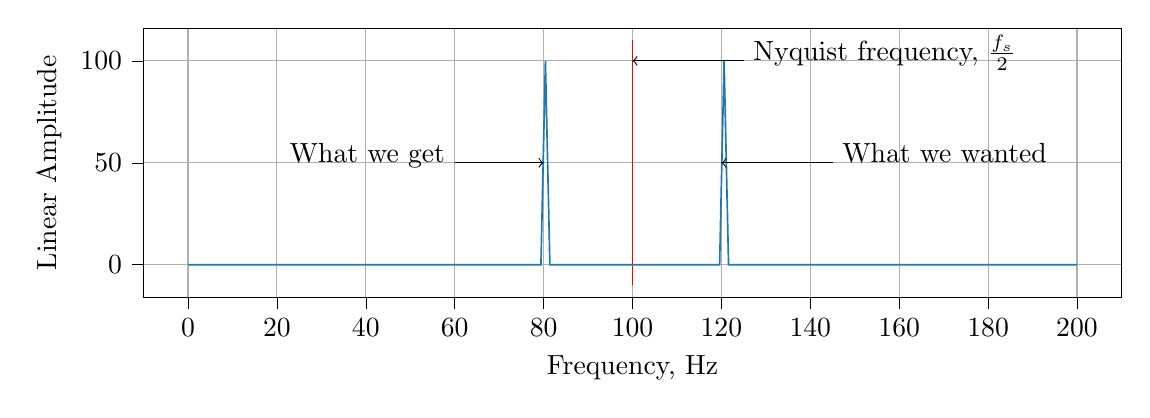
\begin{tikzpicture}

\definecolor{color0}{rgb}{0.12156862745098,0.466666666666667,0.705882352941177}

\begin{axis}[
height=5cm,
legend cell align={left},
legend style={fill opacity=0.8, draw opacity=1, text opacity=1, draw=white!80!black},
tick align=outside,
tick pos=left,
width=14cm,
x grid style={white!69.0196078431373!black},
xlabel={Frequency, Hz},
xmajorgrids,
xmin=-10, xmax=210,
xtick style={color=black},
y grid style={white!69.0196078431373!black},
ylabel={Linear Amplitude},
ymajorgrids,
ymin=-16, ymax=116,
ytick style={color=black}
]
\path [draw=red, semithick]
(axis cs:100,-10)
--(axis cs:100,110);

\addplot [semithick, color0, forget plot]
table {%
0 1.04176496399295e-13
1.00502512562814 1.22852692498498e-13
2.01005025125628 1.64146113790742e-13
3.01507537688442 5.12722440985122e-14
4.02010050251256 1.89635572984625e-13
5.0251256281407 2.09003026072463e-13
6.03015075376884 7.50942547365276e-14
7.03517587939698 3.60288211265824e-13
8.04020100502512 6.61576132530574e-13
9.04522613065327 2.76564554409926e-13
10.0502512562814 1.92358202497402e-13
11.0552763819095 1.01010880236548e-13
12.0603015075377 2.25544214791892e-13
13.0653266331658 1.8719940220499e-13
14.070351758794 1.79054616115051e-13
15.0753768844221 2.85569771117385e-13
16.0804020100502 1.52967228803167e-13
17.0854271356784 1.33152618648232e-13
18.0904522613065 3.25055345582669e-13
19.0954773869347 9.37494207957993e-14
20.1005025125628 7.44324688445693e-14
21.105527638191 1.12008567414346e-13
22.1105527638191 2.01650241098569e-13
23.1155778894472 3.85764507844166e-14
24.1206030150754 1.22134841046306e-13
25.1256281407035 1.77716093122275e-13
26.1306532663317 6.42610827635418e-14
27.1356783919598 1.09930233519008e-13
28.1407035175879 1.00447238321584e-13
29.1457286432161 2.63147928108448e-13
30.1507537688442 2.28054527984479e-14
31.1557788944724 6.16431857761929e-13
32.1608040201005 1.00717425050374e-12
33.1658291457286 6.1437309913277e-13
34.1708542713568 2.15132907111041e-13
35.1758793969849 1.13474426241041e-13
36.1809045226131 1.37983102177136e-13
37.1859296482412 9.96220009144911e-14
38.1909547738693 1.4885545103043e-13
39.1959798994975 5.57427005466418e-14
40.2010050251256 1.96442650341593e-13
41.2060301507538 7.58989451556911e-14
42.2110552763819 1.12263009547582e-13
43.21608040201 1.02050855855012e-13
44.2211055276382 4.47725140338821e-13
45.2261306532663 1.94400582025006e-13
46.2311557788945 2.21580056477014e-13
47.2361809045226 1.06863139747685e-13
48.2412060301507 2.26265351437867e-13
49.2462311557789 2.48590493456595e-13
50.251256281407 1.75879195070945e-13
51.2562814070352 1.86379320904195e-13
52.2613065326633 1.26339595925153e-13
53.2663316582914 3.61765550615109e-13
54.2713567839196 1.26104522344852e-13
55.2763819095477 6.32223321930097e-13
56.2814070351759 2.80114763394157e-13
57.286432160804 3.74598856610979e-13
58.2914572864322 1.83294213991289e-13
59.2964824120603 3.16493249884931e-13
60.3015075376884 1.32348658780032e-13
61.3065326633166 2.93542065695892e-13
62.3115577889447 3.94552579858922e-13
63.3165829145729 5.72370092402213e-13
64.321608040201 3.21950119807266e-13
65.3266331658291 5.95757284561417e-13
66.3316582914573 9.07334943155623e-14
67.3366834170854 4.52510054150999e-13
68.3417085427136 1.98436432015242e-13
69.3467336683417 3.94453972800867e-13
70.3517587939699 2.44419234067847e-13
71.356783919598 2.52377912116451e-13
72.3618090452261 4.94239698060309e-13
73.3668341708543 1.04185395358712e-13
74.3718592964824 3.17340701978095e-13
75.3768844221105 2.86332531789509e-13
76.3819095477387 1.49001844677157e-13
77.3869346733668 1.36394683724063e-13
78.391959798995 3.39880727020675e-14
79.3969849246231 5.07478435387728e-13
80.4020100502512 100
81.4070351758794 4.87193769432429e-13
82.4120603015075 2.61411391347904e-13
83.4170854271357 7.76276232514779e-14
84.4221105527638 3.80535453173215e-13
85.4271356783919 4.62076194956417e-14
86.4321608040201 3.00411173126564e-13
87.4371859296482 3.83741230136667e-13
88.4422110552764 1.00186303096534e-12
89.4472361809045 4.8640340558884e-13
90.4522613065326 3.29485093688873e-13
91.4572864321608 5.57159265566705e-13
92.4623115577889 2.34713721542699e-13
93.4673366834171 9.82265840119626e-14
94.4723618090452 6.23132215485983e-14
95.4773869346734 5.60460276382572e-13
96.4824120603015 5.59103393893974e-13
97.4874371859296 5.26433104938941e-13
98.4924623115578 3.65152025209291e-13
99.4974874371859 3.57935787429034e-13
100.502512562814 1.43399997116854e-13
101.507537688442 3.57935787429034e-13
102.51256281407 3.65152025209291e-13
103.517587939698 5.26433104938941e-13
104.522613065327 5.59103393893974e-13
105.527638190955 5.60460276382572e-13
106.532663316583 6.23132215485983e-14
107.537688442211 9.82265840119626e-14
108.542713567839 2.34713721542699e-13
109.547738693467 5.57159265566705e-13
110.552763819095 3.29485093688873e-13
111.557788944724 4.8640340558884e-13
112.562814070352 1.00186303096534e-12
113.56783919598 3.83741230136667e-13
114.572864321608 3.00411173126564e-13
115.577889447236 4.62076194956416e-14
116.582914572864 3.80535453173215e-13
117.587939698492 7.7627623251478e-14
118.592964824121 2.61411391347904e-13
119.597989949749 4.87193769432429e-13
120.603015075377 100
121.608040201005 5.07478435387728e-13
122.613065326633 3.39880727020675e-14
123.618090452261 1.36394683724063e-13
124.623115577889 1.49001844677157e-13
125.628140703518 2.86332531789509e-13
126.633165829146 3.17340701978095e-13
127.638190954774 1.04185395358712e-13
128.643216080402 4.94239698060309e-13
129.64824120603 2.52377912116451e-13
130.653266331658 2.44419234067847e-13
131.658291457286 3.94453972800867e-13
132.663316582915 1.98436432015242e-13
133.668341708543 4.52510054150999e-13
134.673366834171 9.07334943155623e-14
135.678391959799 5.95757284561417e-13
136.683417085427 3.21950119807266e-13
137.688442211055 5.72370092402213e-13
138.693467336683 3.94552579858922e-13
139.698492462312 2.93542065695892e-13
140.70351758794 1.32348658780032e-13
141.708542713568 3.16493249884931e-13
142.713567839196 1.83294213991289e-13
143.718592964824 3.74598856610979e-13
144.723618090452 2.80114763394157e-13
145.72864321608 6.32223321930097e-13
146.733668341709 1.26104522344852e-13
147.738693467337 3.61765550615109e-13
148.743718592965 1.26339595925153e-13
149.748743718593 1.86379320904195e-13
150.753768844221 1.75879195070945e-13
151.758793969849 2.48590493456595e-13
152.763819095477 2.26265351437866e-13
153.768844221106 1.06863139747685e-13
154.773869346734 2.21580056477014e-13
155.778894472362 1.94400582025006e-13
156.78391959799 4.47725140338821e-13
157.788944723618 1.02050855855012e-13
158.793969849246 1.12263009547582e-13
159.798994974874 7.5898945155691e-14
160.804020100502 1.96442650341593e-13
161.809045226131 5.57427005466417e-14
162.814070351759 1.4885545103043e-13
163.819095477387 9.96220009144911e-14
164.824120603015 1.37983102177136e-13
165.829145728643 1.13474426241041e-13
166.834170854271 2.15132907111041e-13
167.839195979899 6.14373099132769e-13
168.844221105528 1.00717425050374e-12
169.849246231156 6.16431857761929e-13
170.854271356784 2.28054527984479e-14
171.859296482412 2.63147928108448e-13
172.86432160804 1.00447238321584e-13
173.869346733668 1.09930233519008e-13
174.874371859296 6.42610827635418e-14
175.879396984925 1.77716093122275e-13
176.884422110553 1.22134841046306e-13
177.889447236181 3.85764507844166e-14
178.894472361809 2.01650241098569e-13
179.899497487437 1.12008567414346e-13
180.904522613065 7.44324688445693e-14
181.909547738693 9.37494207957992e-14
182.914572864322 3.25055345582669e-13
183.91959798995 1.33152618648232e-13
184.924623115578 1.52967228803167e-13
185.929648241206 2.85569771117385e-13
186.934673366834 1.79054616115051e-13
187.939698492462 1.8719940220499e-13
188.94472361809 2.25544214791892e-13
189.949748743719 1.01010880236548e-13
190.954773869347 1.92358202497402e-13
191.959798994975 2.76564554409926e-13
192.964824120603 6.61576132530574e-13
193.969849246231 3.60288211265824e-13
194.974874371859 7.50942547365277e-14
195.979899497487 2.09003026072463e-13
196.984924623116 1.89635572984625e-13
197.989949748744 5.12722440985122e-14
198.994974874372 1.64146113790741e-13
200 1.22852692498498e-13
};
\draw[->,draw=black] (axis cs:125,100) -- (axis cs:100,100);
\draw (axis cs:125,100) node[
  scale=1,
  anchor=base west,
  text=black,
  rotate=0.0
]{Nyquist frequency, $\frac{f_s}{2}$};
\draw[->,draw=black] (axis cs:145,50) -- (axis cs:120,50);
\draw (axis cs:145,50) node[
  scale=1,
  anchor=base west,
  text=black,
  rotate=0.0
]{What we wanted};
\draw[->,draw=black] (axis cs:60,50) -- (axis cs:80,50);
\draw (axis cs:60,50) node[
  scale=1,
  anchor=base east,
  text=black,
  rotate=0.0
]{What we get};
\end{axis}

\end{tikzpicture}

		% \includegraphics[width = \textwidth]{aliasingFreqDomain.png}
		\caption[Aliasing in the Frequency Domain]
		{Here we can see the phenomenon of aliasing in the frequency domain. We try to synthesize a sine wave at 120Hz. At a sampling rate of 200 Hz, this is not possible, nyquist is at 100 Hz. What we actually get is a sine wave at about 80Hz. In this plot, the nyquist frequency is marked with the red line. Please note that the distance between the red line to both peaks is identical. This is why the phenomenon is also called \textit{fold-back}.}
		\label{fig:aliasingFreqDomain}
	\end{center}
\end{figure}


But how is the aliased frequency calculated? To get a correct result also if you go 2 or more times past the Nyquist frequency, and still be correct in phase, please look at \link{https://colab.research.google.com/drive/10NRGmmLRGxy\_3j7ecGKcME0gkQKmCDOW}{this Notebook}. For the case where we go only once over the Nyquist Frequency we can just calculate:

\begin{equation}
	f_a = f_s-f_o
\end{equation}
Where $f_a$ is the Frequency we will hear, $f_o$ is the intended frequency and $f_s$ is the sampling rate. 
\bgInfo{
For cases where we pass Nyquist multiple times things start to get a bit complicated. In case we went over Nyquist odd times we can use the following Equation making use of the modulo. That is this equation os valid between $f_n$ and $f_s=2f_n$, between $3f_n$ and $4f_n$ and so on:


\begin{equation}
	f_a = (fs-f_o) mod  \frac{f_s}{2}
\end{equation}

otherwise we have to use the following Equation:
\begin{equation}
	f_a = f_o mod  \frac{f_s}{2}
\end{equation}

}

\section{Scaling and Mapping Signals}
It is an important skill to be able to scale signals from one range to another. We need it a lot and we will be able to think about signals more easily if we mastered this task. It's actually quite simple, we just have to imagine the signals visually.\\
So what exactly do we have to do here? We are confronted with the following problem: Given some signal, say, a sine wave with its maximum at the value 1 and its minimum at the value -1. How to bring it to a different range, say, 0-10?\\
It helps me a lot to solve this problem in two parts: first get the input in the range 0-1, then from there go to the desired range. What can we do to the signal? Let's take a sine wave like the one in Figure ~\ref{fig:aSine}. Well we can add and subtract to move the wave vertically, so let's add 1 to move it up, have a look at Figure~\ref{fig:aShiftedSine}.

\begin{figure}[H]
	\centering
	% This file was created with tikzplotlib v0.9.14.
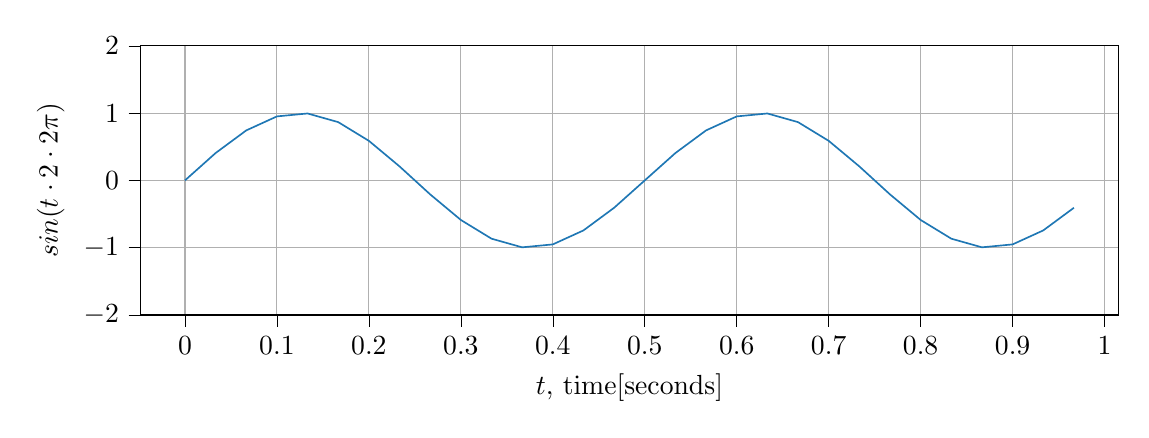
\begin{tikzpicture}

\definecolor{color0}{rgb}{0.12156862745098,0.466666666666667,0.705882352941177}

\begin{axis}[
height=5cm,
tick align=outside,
tick pos=left,
width=14cm,
x grid style={white!69.0196078431373!black},
xlabel={\(\displaystyle t\), time[seconds]},
xmajorgrids,
xmin=-0.0483333333333333, xmax=1.015,
xtick style={color=black},
y grid style={white!69.0196078431373!black},
ylabel={\(\displaystyle sin(t \cdot 2 \cdot 2 \pi)\)},
ymajorgrids,
ymin=-2, ymax=2,
ytick style={color=black}
]
\addplot [semithick, color0]
table {%
0 0
0.0333333333333333 0.4067366430758
0.0666666666666667 0.743144825477394
0.1 0.951056516295154
0.133333333333333 0.994521895368273
0.166666666666667 0.866025403784439
0.2 0.587785252292473
0.233333333333333 0.207911690817759
0.266666666666667 -0.207911690817759
0.3 -0.587785252292473
0.333333333333333 -0.866025403784438
0.366666666666667 -0.994521895368273
0.4 -0.951056516295154
0.433333333333333 -0.743144825477394
0.466666666666667 -0.4067366430758
0.5 -2.44929359829471e-16
0.533333333333333 0.4067366430758
0.566666666666667 0.743144825477394
0.6 0.951056516295154
0.633333333333333 0.994521895368273
0.666666666666667 0.866025403784439
0.7 0.587785252292473
0.733333333333333 0.207911690817761
0.766666666666667 -0.20791169081776
0.8 -0.587785252292473
0.833333333333333 -0.866025403784439
0.866666666666667 -0.994521895368273
0.9 -0.951056516295154
0.933333333333333 -0.743144825477394
0.966666666666667 -0.406736643075801
};
\end{axis}

\end{tikzpicture}

	% \includegraphics[width=11cm]{stdSine.png}
	\caption[a sine wave, $f=2Hz$]
	{a sine wave, $f=2Hz$}
	\label{fig:aSine}
\end{figure}

\begin{figure}[H]
	\centering
	% This file was created with tikzplotlib v0.9.14.
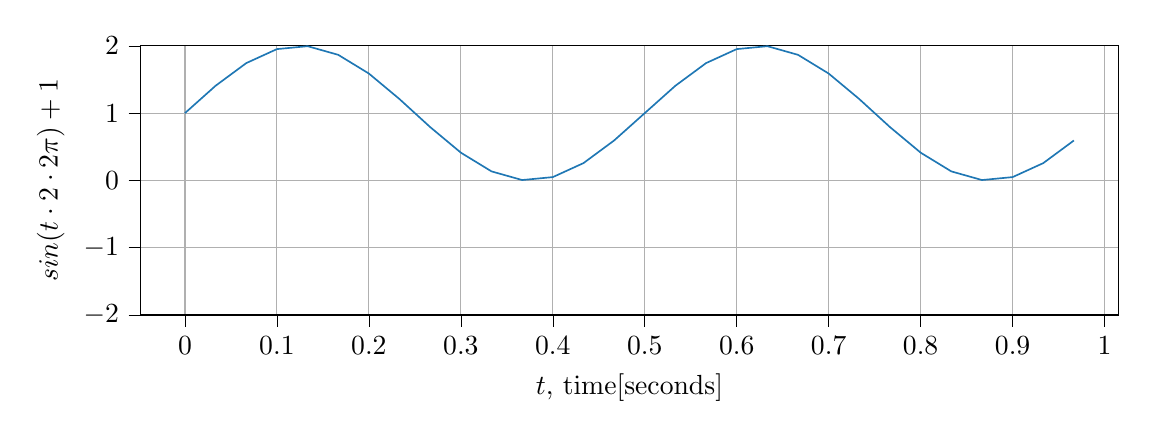
\begin{tikzpicture}

\definecolor{color0}{rgb}{0.12156862745098,0.466666666666667,0.705882352941177}

\begin{axis}[
height=5cm,
tick align=outside,
tick pos=left,
width=14cm,
x grid style={white!69.0196078431373!black},
xlabel={\(\displaystyle t\), time[seconds]},
xmajorgrids,
xmin=-0.0483333333333333, xmax=1.015,
xtick style={color=black},
y grid style={white!69.0196078431373!black},
ylabel={\(\displaystyle sin(t \cdot 2 \cdot 2 \pi) + 1\)},
ymajorgrids,
ymin=-2, ymax=2,
ytick style={color=black}
]
\addplot [semithick, color0]
table {%
0 1
0.0333333333333333 1.4067366430758
0.0666666666666667 1.74314482547739
0.1 1.95105651629515
0.133333333333333 1.99452189536827
0.166666666666667 1.86602540378444
0.2 1.58778525229247
0.233333333333333 1.20791169081776
0.266666666666667 0.792088309182241
0.3 0.412214747707527
0.333333333333333 0.133974596215562
0.366666666666667 0.00547810463172671
0.4 0.0489434837048464
0.433333333333333 0.256855174522606
0.466666666666667 0.5932633569242
0.5 1
0.533333333333333 1.4067366430758
0.566666666666667 1.74314482547739
0.6 1.95105651629515
0.633333333333333 1.99452189536827
0.666666666666667 1.86602540378444
0.7 1.58778525229247
0.733333333333333 1.20791169081776
0.766666666666667 0.79208830918224
0.8 0.412214747707527
0.833333333333333 0.133974596215561
0.866666666666667 0.0054781046317266
0.9 0.0489434837048462
0.933333333333333 0.256855174522606
0.966666666666667 0.593263356924199
};
\end{axis}

\end{tikzpicture}

	% \includegraphics[width=11cm]{sinePlusOne.png}
	\caption[a sine wave plus 1]
	{the same sine wave, $f=2Hz$, 1 added to a each sample, therefore shifted upwards.}
	\label{fig:aShiftedSine}
\end{figure}

So we can move signals around by adding constant values. We can scale them by multiplication. So if we take our sine that now ranges from 0 to 2 and multiply it by 0.5, we get whats in figure \ref{fig:sine01}.

\begin{figure}[H]
 	\centering
 	% \includegraphics[width=11cm]{sine01.png}
 	% This file was created with tikzplotlib v0.9.14.
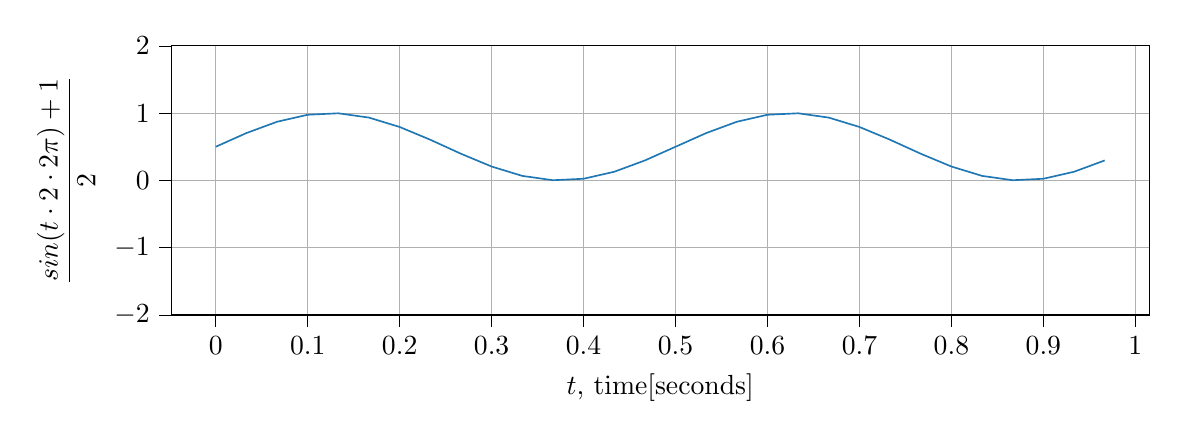
\begin{tikzpicture}

\definecolor{color0}{rgb}{0.12156862745098,0.466666666666667,0.705882352941177}

\begin{axis}[
height=5cm,
tick align=outside,
tick pos=left,
width=14cm,
x grid style={white!69.0196078431373!black},
xlabel={\(\displaystyle t\), time[seconds]},
xmajorgrids,
xmin=-0.0483333333333333, xmax=1.015,
xtick style={color=black},
y grid style={white!69.0196078431373!black},
ylabel={\(\displaystyle \frac{sin(t \cdot 2 \cdot 2 \pi) + 1}{2}\)},
ymajorgrids,
ymin=-2, ymax=2,
ytick style={color=black}
]
\addplot [semithick, color0]
table {%
0 0.5
0.0333333333333333 0.7033683215379
0.0666666666666667 0.871572412738697
0.1 0.975528258147577
0.133333333333333 0.997260947684137
0.166666666666667 0.933012701892219
0.2 0.793892626146237
0.233333333333333 0.60395584540888
0.266666666666667 0.39604415459112
0.3 0.206107373853763
0.333333333333333 0.0669872981077808
0.366666666666667 0.00273905231586336
0.4 0.0244717418524232
0.433333333333333 0.128427587261303
0.466666666666667 0.2966316784621
0.5 0.5
0.533333333333333 0.7033683215379
0.566666666666667 0.871572412738697
0.6 0.975528258147577
0.633333333333333 0.997260947684137
0.666666666666667 0.93301270189222
0.7 0.793892626146237
0.733333333333333 0.60395584540888
0.766666666666667 0.39604415459112
0.8 0.206107373853764
0.833333333333333 0.0669872981077806
0.866666666666667 0.0027390523158633
0.9 0.0244717418524231
0.933333333333333 0.128427587261303
0.966666666666667 0.296631678462099
};
\end{axis}

\end{tikzpicture}

 	\caption[sine 0 to 1]
 	{Sine, $f=2Hz$, with a range of 0-1. Obtained by taking a sine wave, adding 1 and dividing by two afterwards.}
 	\label{fig:sine01}
 \end{figure}

\hspace{1cm}

Using what we got now in figure \ref{fig:sine01}, we can just multiply by 10, easy! Beware that there are always multiple solutions to this kind of a problem. Try to find another one for the problem above!

\begin{question}
Let's take a sine wave that has it's minimum at 2 and it's maximum at 5. What do we have to do to get it into a -1 to 1 range?
\end{question}
\begin{Answer}
We could subtract 3.5 to center the wave around zero first. Afterwards we take care of the amplitude by multiplying by $\frac{2}{3}$ (since the initial wave has a peak-to-peak amplitude of three and we want a peak-to-peak amplitude of 2)
\end{Answer}



\section{What's DC-Offset?}

What we did above by adding a constant value to a signal can be called adding DC-offset (``Gleichspannungsversatz''), DC-Bias or a DC component. These are different words for the same thing.\\
DC-offset can also be encountered in signals we recorded (caused by old or broken equipment mainly). But we have seen that we can also generate DC-offset.\\
To state it again clearly:
\begin{framed}
DC-Offset is a constant value over time, or a constant offset from the zero value in Y. So for example in figure \ref{fig:sine01} we see a DC-offset of 0.5 since subtracting this value would center the wave around 0.
\end{framed}
If we try to think how this kind of signal looks in the frequency domain we find that it is energy at 0Hz. In figure \ref{fig:dcViz} you can see a couple of cosine waves plotted. This should hep imagine that a constant signal, a signal that does not move a all, can be described by a cosine with 0 Hz and a certain amplitude.

\begin{figure}[h!]
	\centering
	% This file was created with tikzplotlib v0.9.14.
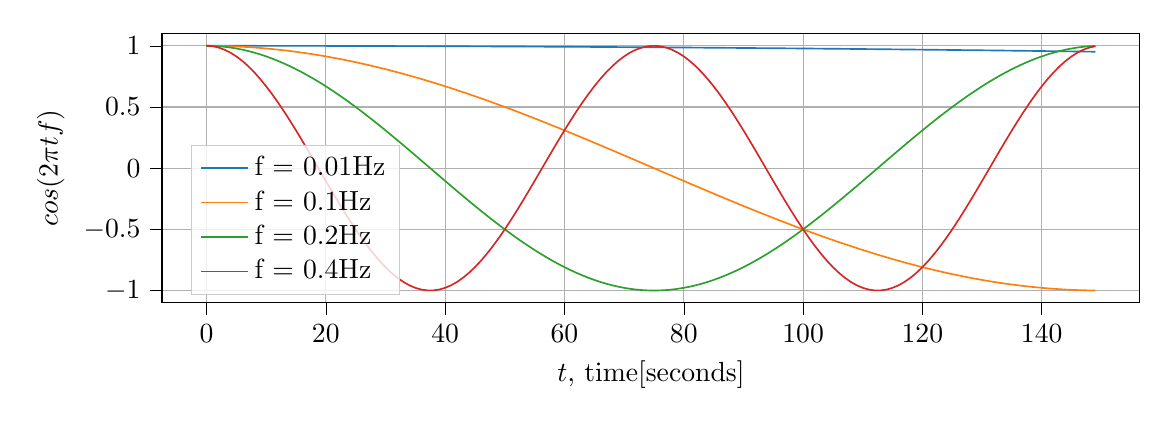
\begin{tikzpicture}

\definecolor{color0}{rgb}{0.12156862745098,0.466666666666667,0.705882352941177}
\definecolor{color1}{rgb}{1,0.498039215686275,0.0549019607843137}
\definecolor{color2}{rgb}{0.172549019607843,0.627450980392157,0.172549019607843}
\definecolor{color3}{rgb}{0.83921568627451,0.152941176470588,0.156862745098039}

\begin{axis}[
height=5cm,
legend cell align={left},
legend style={
  fill opacity=0.8,
  draw opacity=1,
  text opacity=1,
  at={(0.03,0.03)},
  anchor=south west,
  draw=white!80!black
},
tick align=outside,
tick pos=left,
width=14cm,
x grid style={white!69.0196078431373!black},
xlabel={\(\displaystyle t\), time[seconds]},
xmajorgrids,
xmin=-7.45, xmax=156.45,
xtick style={color=black},
y grid style={white!69.0196078431373!black},
ylabel={\(\displaystyle cos(2 \pi t f)\)},
ymajorgrids,
ymin=-1.1, ymax=1.1,
ytick style={color=black}
]
\addplot [semithick, color0]
table {%
0 1
1 0.999997806755379
2 0.999991227031138
3 0.999980260856137
4 0.999964908278481
5 0.999945169365512
6 0.999921044203816
7 0.999892532899217
8 0.99985963557678
9 0.999822352380809
10 0.999780683474845
11 0.99973462904167
12 0.9996841892833
13 0.999629364420989
14 0.999570154695225
15 0.999506560365732
16 0.999438581711464
17 0.999366219030611
18 0.999289472640589
19 0.999208342878047
20 0.999122830098858
21 0.999032934678125
22 0.998938657010171
23 0.998839997508546
24 0.998736956606017
25 0.998629534754574
26 0.99851773242542
27 0.998401550108975
28 0.998280988314872
29 0.998156047571954
30 0.998026728428272
31 0.997893031451082
32 0.997754957226847
33 0.997612506361225
34 0.997465679479078
35 0.997314477224458
36 0.997158900260614
37 0.996998949269982
38 0.996834624954185
39 0.99666592803403
40 0.996492859249504
41 0.996315419359773
42 0.996133609143173
43 0.995947429397213
44 0.995756880938569
45 0.99556196460308
46 0.995362681245744
47 0.995159031740715
48 0.9949510169813
49 0.994738637879953
50 0.994521895368273
51 0.994300790396999
52 0.994075323936005
53 0.993845496974297
54 0.993611310520008
55 0.993372765600396
56 0.993129863261835
57 0.992882604569814
58 0.992630990608929
59 0.992375022482883
60 0.992114701314478
61 0.991850028245609
62 0.991581004437262
63 0.991307631069507
64 0.991029909341493
65 0.990747840471444
66 0.990461425696651
67 0.990170666273471
68 0.989875563477316
69 0.989576118602651
70 0.989272332962988
71 0.98896420789088
72 0.988651744737914
73 0.988334944874706
74 0.988013809690895
75 0.987688340595138
76 0.9873585390151
77 0.987024406397454
78 0.986685944207868
79 0.986343153931003
80 0.985996037070505
81 0.985644595148998
82 0.985288829708079
83 0.984928742308308
84 0.984564334529205
85 0.984195607969242
86 0.983822564245833
87 0.98344520499533
88 0.983063531873015
89 0.982677546553095
90 0.982287250728689
91 0.981892646111825
92 0.981493734433433
93 0.981090517443334
94 0.980682996910236
95 0.980271174621722
96 0.979855052384247
97 0.979434632023126
98 0.97900991538253
99 0.978580904325472
100 0.978147600733806
101 0.977710006508212
102 0.977268123568193
103 0.976821953852065
104 0.976371499316945
105 0.975916761938747
106 0.975457743712173
107 0.9749944466507
108 0.974526872786577
109 0.974055024170811
110 0.97357890287316
111 0.973098510982127
112 0.972613850604944
113 0.972124923867569
114 0.971631732914674
115 0.971134279909636
116 0.970632567034527
117 0.970126596490106
118 0.969616370495806
119 0.969101891289729
120 0.968583161128631
121 0.968060182287918
122 0.96753295706163
123 0.967001487762435
124 0.966465776721618
125 0.965925826289068
126 0.965381638833274
127 0.964833216741307
128 0.964280562418815
129 0.96372367829001
130 0.963162566797658
131 0.96259723040307
132 0.962027671586086
133 0.961453892845071
134 0.960875896696899
135 0.960293685676943
136 0.959707262339067
137 0.959116629255609
138 0.958521789017376
139 0.957922744233627
140 0.957319497532067
141 0.95671205155883
142 0.956100408978472
143 0.955484572473956
144 0.954864544746643
145 0.954240328516277
146 0.953611926520976
147 0.952979341517219
148 0.952342576279833
149 0.951701633601982
};
\addlegendentry{f = 0.01Hz}
\addplot [semithick, color1]
table {%
0 1
1 0.999780683474845
2 0.999122830098858
3 0.998026728428272
4 0.996492859249504
5 0.994521895368273
6 0.992114701314478
7 0.989272332962988
8 0.985996037070505
9 0.982287250728689
10 0.978147600733806
11 0.97357890287316
12 0.968583161128631
13 0.963162566797658
14 0.957319497532067
15 0.951056516295154
16 0.944376370237481
17 0.937281989491892
18 0.929776485888251
19 0.921863151588501
20 0.913545457642601
21 0.90482705246602
22 0.895711760239413
23 0.886203579231215
24 0.876306680043864
25 0.866025403784439
26 0.855364260160507
27 0.844327925502015
28 0.832921240710099
29 0.821149209133704
30 0.809016994374947
31 0.796529918024196
32 0.78369345732584
33 0.770513242775789
34 0.756995055651756
35 0.743144825477394
36 0.728968627421412
37 0.714472679632803
38 0.699663340513365
39 0.684547105928689
40 0.669130606358858
41 0.653420603990105
42 0.63742398974869
43 0.62114778027831
44 0.604599114862375
45 0.587785252292473
46 0.570713567684432
47 0.553391549243344
48 0.535826794978997
49 0.51802700937313
50 0.5
51 0.481753674101715
52 0.463296035119862
53 0.444635179184928
54 0.425779291565073
55 0.4067366430758
56 0.387515586452103
57 0.368124552684678
58 0.348572047321815
59 0.328866646738583
60 0.309016994374947
61 0.289031796944472
62 0.268919820615266
63 0.248689887164855
64 0.228350870110656
65 0.207911690817759
66 0.187381314585725
67 0.166768746716102
68 0.146083028562412
69 0.125333233564304
70 0.104528463267653
71 0.0836778433323154
72 0.0627905195293133
73 0.0418756537291997
74 0.0209424198833568
75 6.12323399573677e-17
76 -0.0209424198833569
77 -0.0418756537291998
78 -0.0627905195293134
79 -0.0836778433323155
80 -0.104528463267653
81 -0.125333233564304
82 -0.146083028562412
83 -0.166768746716102
84 -0.187381314585725
85 -0.20791169081776
86 -0.228350870110656
87 -0.248689887164855
88 -0.268919820615266
89 -0.289031796944472
90 -0.309016994374947
91 -0.328866646738583
92 -0.348572047321815
93 -0.368124552684678
94 -0.387515586452103
95 -0.4067366430758
96 -0.425779291565073
97 -0.444635179184928
98 -0.463296035119862
99 -0.481753674101715
100 -0.5
101 -0.51802700937313
102 -0.535826794978996
103 -0.553391549243344
104 -0.570713567684432
105 -0.587785252292473
106 -0.604599114862375
107 -0.621147780278311
108 -0.63742398974869
109 -0.653420603990105
110 -0.669130606358858
111 -0.684547105928689
112 -0.699663340513365
113 -0.714472679632803
114 -0.728968627421412
115 -0.743144825477394
116 -0.756995055651756
117 -0.770513242775789
118 -0.78369345732584
119 -0.796529918024196
120 -0.809016994374947
121 -0.821149209133704
122 -0.832921240710099
123 -0.844327925502015
124 -0.855364260160507
125 -0.866025403784439
126 -0.876306680043864
127 -0.886203579231215
128 -0.895711760239413
129 -0.90482705246602
130 -0.913545457642601
131 -0.9218631515885
132 -0.929776485888251
133 -0.937281989491892
134 -0.944376370237481
135 -0.951056516295154
136 -0.957319497532067
137 -0.963162566797658
138 -0.968583161128631
139 -0.97357890287316
140 -0.978147600733806
141 -0.982287250728689
142 -0.985996037070505
143 -0.989272332962988
144 -0.992114701314478
145 -0.994521895368273
146 -0.996492859249504
147 -0.998026728428272
148 -0.999122830098858
149 -0.999780683474845
};
\addlegendentry{f = 0.1Hz}
\addplot [semithick, color2]
table {%
0 1
1 0.999122830098858
2 0.996492859249504
3 0.992114701314478
4 0.985996037070505
5 0.978147600733806
6 0.968583161128631
7 0.957319497532067
8 0.944376370237481
9 0.929776485888251
10 0.913545457642601
11 0.895711760239413
12 0.876306680043864
13 0.855364260160507
14 0.832921240710099
15 0.809016994374947
16 0.78369345732584
17 0.756995055651756
18 0.728968627421412
19 0.699663340513365
20 0.669130606358858
21 0.63742398974869
22 0.604599114862375
23 0.570713567684432
24 0.535826794978997
25 0.5
26 0.463296035119862
27 0.425779291565073
28 0.387515586452103
29 0.348572047321815
30 0.309016994374947
31 0.268919820615266
32 0.228350870110656
33 0.187381314585725
34 0.146083028562412
35 0.104528463267653
36 0.0627905195293133
37 0.0209424198833568
38 -0.0209424198833569
39 -0.0627905195293134
40 -0.104528463267653
41 -0.146083028562412
42 -0.187381314585725
43 -0.228350870110656
44 -0.268919820615266
45 -0.309016994374947
46 -0.348572047321815
47 -0.387515586452103
48 -0.425779291565073
49 -0.463296035119862
50 -0.5
51 -0.535826794978996
52 -0.570713567684432
53 -0.604599114862375
54 -0.63742398974869
55 -0.669130606358858
56 -0.699663340513365
57 -0.728968627421412
58 -0.756995055651756
59 -0.78369345732584
60 -0.809016994374947
61 -0.832921240710099
62 -0.855364260160507
63 -0.876306680043864
64 -0.895711760239413
65 -0.913545457642601
66 -0.929776485888251
67 -0.944376370237481
68 -0.957319497532067
69 -0.968583161128631
70 -0.978147600733806
71 -0.985996037070505
72 -0.992114701314478
73 -0.996492859249504
74 -0.999122830098858
75 -1
76 -0.999122830098858
77 -0.996492859249504
78 -0.992114701314478
79 -0.985996037070505
80 -0.978147600733806
81 -0.968583161128631
82 -0.957319497532067
83 -0.944376370237481
84 -0.929776485888251
85 -0.913545457642601
86 -0.895711760239413
87 -0.876306680043864
88 -0.855364260160507
89 -0.832921240710099
90 -0.809016994374947
91 -0.78369345732584
92 -0.756995055651756
93 -0.728968627421412
94 -0.699663340513365
95 -0.669130606358858
96 -0.63742398974869
97 -0.604599114862375
98 -0.570713567684432
99 -0.535826794978996
100 -0.5
101 -0.463296035119862
102 -0.425779291565073
103 -0.387515586452103
104 -0.348572047321815
105 -0.309016994374948
106 -0.268919820615266
107 -0.228350870110655
108 -0.187381314585725
109 -0.146083028562412
110 -0.104528463267653
111 -0.0627905195293132
112 -0.0209424198833567
113 0.0209424198833564
114 0.0627905195293137
115 0.104528463267654
116 0.146083028562411
117 0.187381314585725
118 0.228350870110655
119 0.268919820615266
120 0.309016994374947
121 0.348572047321815
122 0.387515586452103
123 0.425779291565072
124 0.463296035119862
125 0.500000000000001
126 0.535826794978997
127 0.570713567684432
128 0.604599114862375
129 0.63742398974869
130 0.669130606358858
131 0.699663340513365
132 0.728968627421412
133 0.756995055651757
134 0.78369345732584
135 0.809016994374947
136 0.832921240710099
137 0.855364260160507
138 0.876306680043863
139 0.895711760239413
140 0.913545457642601
141 0.929776485888251
142 0.944376370237481
143 0.957319497532067
144 0.968583161128631
145 0.978147600733806
146 0.985996037070505
147 0.992114701314478
148 0.996492859249504
149 0.999122830098858
};
\addlegendentry{f = 0.2Hz}
\addplot [semithick, color3]
table {%
0 1
1 0.996492859249504
2 0.985996037070505
3 0.968583161128631
4 0.944376370237481
5 0.913545457642601
6 0.876306680043864
7 0.832921240710099
8 0.78369345732584
9 0.728968627421412
10 0.669130606358858
11 0.604599114862375
12 0.535826794978997
13 0.463296035119862
14 0.387515586452103
15 0.309016994374947
16 0.228350870110656
17 0.146083028562412
18 0.0627905195293133
19 -0.0209424198833569
20 -0.104528463267653
21 -0.187381314585725
22 -0.268919820615266
23 -0.348572047321815
24 -0.425779291565073
25 -0.5
26 -0.570713567684432
27 -0.63742398974869
28 -0.699663340513365
29 -0.756995055651756
30 -0.809016994374947
31 -0.855364260160507
32 -0.895711760239413
33 -0.929776485888251
34 -0.957319497532067
35 -0.978147600733806
36 -0.992114701314478
37 -0.999122830098858
38 -0.999122830098858
39 -0.992114701314478
40 -0.978147600733806
41 -0.957319497532067
42 -0.929776485888251
43 -0.895711760239413
44 -0.855364260160507
45 -0.809016994374947
46 -0.756995055651756
47 -0.699663340513365
48 -0.63742398974869
49 -0.570713567684432
50 -0.5
51 -0.425779291565073
52 -0.348572047321815
53 -0.268919820615266
54 -0.187381314585725
55 -0.104528463267653
56 -0.0209424198833567
57 0.0627905195293137
58 0.146083028562411
59 0.228350870110655
60 0.309016994374947
61 0.387515586452103
62 0.463296035119862
63 0.535826794978997
64 0.604599114862375
65 0.669130606358858
66 0.728968627421412
67 0.78369345732584
68 0.832921240710099
69 0.876306680043863
70 0.913545457642601
71 0.944376370237481
72 0.968583161128631
73 0.985996037070505
74 0.996492859249504
75 1
76 0.996492859249504
77 0.985996037070505
78 0.968583161128631
79 0.944376370237481
80 0.913545457642601
81 0.876306680043863
82 0.832921240710099
83 0.78369345732584
84 0.728968627421412
85 0.669130606358858
86 0.604599114862375
87 0.535826794978996
88 0.463296035119862
89 0.387515586452102
90 0.309016994374948
91 0.228350870110657
92 0.146083028562411
93 0.0627905195293133
94 -0.0209424198833571
95 -0.104528463267653
96 -0.187381314585725
97 -0.268919820615266
98 -0.348572047321814
99 -0.425779291565073
100 -0.500000000000001
101 -0.570713567684431
102 -0.637423989748689
103 -0.699663340513365
104 -0.756995055651757
105 -0.809016994374947
106 -0.855364260160506
107 -0.895711760239414
108 -0.929776485888251
109 -0.957319497532067
110 -0.978147600733806
111 -0.992114701314478
112 -0.999122830098858
113 -0.999122830098858
114 -0.992114701314478
115 -0.978147600733805
116 -0.957319497532067
117 -0.929776485888251
118 -0.895711760239413
119 -0.855364260160506
120 -0.809016994374948
121 -0.756995055651757
122 -0.699663340513366
123 -0.637423989748691
124 -0.570713567684432
125 -0.499999999999998
126 -0.425779291565072
127 -0.348572047321815
128 -0.268919820615265
129 -0.187381314585724
130 -0.104528463267654
131 -0.0209424198833579
132 0.0627905195293144
133 0.146083028562413
134 0.228350870110657
135 0.309016994374947
136 0.387515586452103
137 0.463296035119862
138 0.535826794978995
139 0.604599114862375
140 0.66913060635886
141 0.728968627421412
142 0.78369345732584
143 0.8329212407101
144 0.876306680043864
145 0.9135454576426
146 0.944376370237481
147 0.968583161128631
148 0.985996037070505
149 0.996492859249504
};
\addlegendentry{f = 0.4Hz}
\end{axis}

\end{tikzpicture}

	% \includegraphics[width=11cm]{dcOffsetViz}
	\caption[Cosines to DC]
	{Cosines with different very low frequencies approaching 0Hz, so DC offset.}
	\label{fig:dcViz}
\end{figure}

Let's quickly state this differently, so we can appreciate the surprising connections between DC-offset and an impulse. A DC-offset signal is a signal consisting of constant values, so for example $\{...,1,1,1,1,1,1,...\}$. Its spectrum is a single peak at 0Hz, so the spectrum's values look like $\{..., 0,0,0,1,0,0,0,...\}$\footnote{Why is the $1$, so the 0 Hz component not at the beginning of the list? Or is it not 0 Hz? The 1 is supposed to be at 0Hz, and it is centered in this list because doing an FFT actually always gets us a two-sided spectrum. You can ignore this fact until the FFT chapter, and pretend that the list starts with 1 (which wouldn't be wrong also). }


\begin{figure}[H]
	\begin{center}
		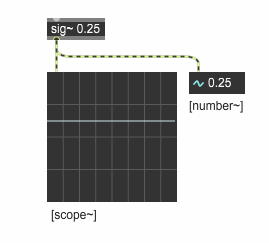
\includegraphics{dcPd.png}
		\caption[Dc-offset in Max]
		{One of the ways to generate a DC signal in Max.}
		\label{fig:dcOffsetPD}
	\end{center}
\end{figure}




% \comm{explanations and visualizations missing}

\section{What's an Impulse?}

Impulses are very useful signals. We can produce an impulse using the \pd{click\textasciitilde} object.

\begin{figure}[H]
	\begin{center}
		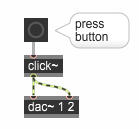
\includegraphics{dirac.png}
		\caption[The click object]
		{The \pd{click\textasciitilde} object produces an impulse if we send it a \texttt{bang}.}
		\label{fig:impulseInPd}
	\end{center}
\end{figure}
\bgInfo{
Different people will define what's an impulse in different ways:
\begin{itemize}
	\item A sound engineer might tell you, that clapping your hands or shooting with a gun creates an impulse
	\item a mathematician will maybe give you the definition of the \textit{dirac delta function}. A dirac function is a continuous function having infinite height and being infinitely short. Its integral (area under the curve) is 1.
	\item Somebody working with discrete (so digital) signals will give you rather the definition of the Kronecker delta function\footnote{It's very common and kind of wrong to call digital impulses "dirac functions" or "dirac impulses". Sometimes people like to use "big" words. So instead of saying "impulse", they say "dirac delta function". Dirac delta functions have importance in mathematics and analysis. But since they have infinite value and are infinitely short they can't exist in reality. They are a theoretical idea. Therefore, more often than not, the term is used a bit incorrectly in an audio context.}:
	\begin{equation}
		\delta(i) = \begin{cases}
0, & \mbox{if } i \ne 0  \\
1, & \mbox{if } i=0 \end{cases}
	\end{equation}
\end{itemize}


}

For us, strictly speaking, an impulse will be a signal that contains only zeros, but one sample with the value one (so we will mean the Kronecker delta function if we say 'impulse'). We can see such an impulse in figure \ref{fig:unitImpulse}. On the x-axis, we have the time in samples\footnote{Don't be irritated by the fact that the sample numbers on the x-axis are ranging from $-5$ to $5$. You can just as well imagine them going from 0 to 10 or 1 to 11. It doesn't really matter. However, this way of displaying an impulse is very common since if the impulse is filtered, it's symmetry is an important factor.}.


\begin{figure}[H]
	\begin{center}
		% This file was created with tikzplotlib v0.9.14.
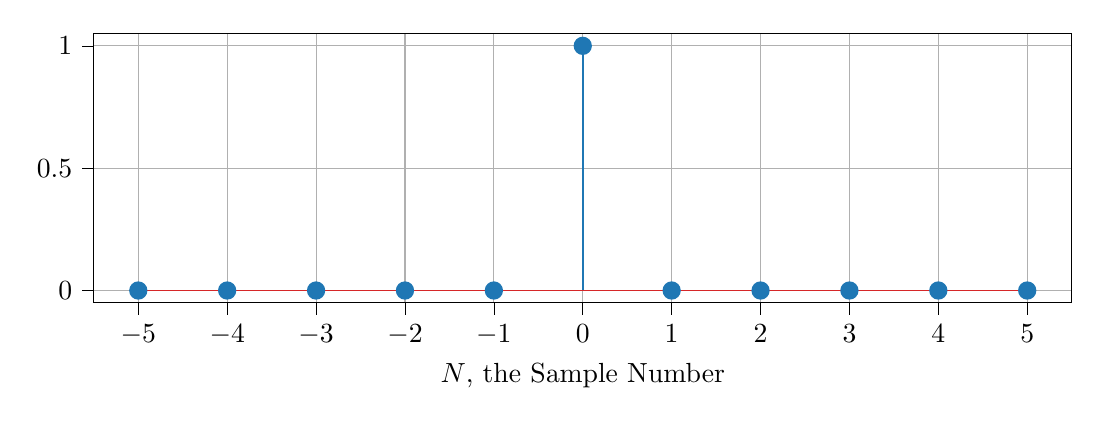
\begin{tikzpicture}

\definecolor{color0}{rgb}{0.12156862745098,0.466666666666667,0.705882352941177}
\definecolor{color1}{rgb}{0.83921568627451,0.152941176470588,0.156862745098039}

\begin{axis}[
height=5cm,
tick align=outside,
tick pos=left,
width=14cm,
x grid style={white!69.0196078431373!black},
xlabel={\(\displaystyle N\), the Sample Number },
xmajorgrids,
xmin=-5.5, xmax=5.5,
xtick style={color=black},
y grid style={white!69.0196078431373!black},
ymajorgrids,
ymin=-0.05, ymax=1.05,
ytick style={color=black}
]
\addplot [semithick, color0]
table {%
-5 0
-5 0
};
\addplot [semithick, color0]
table {%
-4 0
-4 0
};
\addplot [semithick, color0]
table {%
-3 0
-3 0
};
\addplot [semithick, color0]
table {%
-2 0
-2 0
};
\addplot [semithick, color0]
table {%
-1 0
-1 0
};
\addplot [semithick, color0]
table {%
0 0
0 1
};
\addplot [semithick, color0]
table {%
1 0
1 0
};
\addplot [semithick, color0]
table {%
2 0
2 0
};
\addplot [semithick, color0]
table {%
3 0
3 0
};
\addplot [semithick, color0]
table {%
4 0
4 0
};
\addplot [semithick, color0]
table {%
5 0
5 0
};
\addplot [semithick, color0, mark=*, mark size=3, mark options={solid}, only marks]
table {%
-5 0
-4 0
-3 0
-2 0
-1 0
0 1
1 0
2 0
3 0
4 0
5 0
};
\addplot [semithick, color1]
table {%
-5 0
5 0
};
\end{axis}

\end{tikzpicture}

		% \includegraphics[width = \textwidth]{unitImpulse.png}
		\caption{The unit impulse function.}
		\label{fig:unitImpulse}
	\end{center}
\end{figure}

So in the time domain, an impulse's samples have the values $\{...,0,0,0,1,0,0,0,...\}$. If we look at it's spectrum, we will find that it contains all frequencies, there is just a flat line in the spectrum (you can see an impulse's spectrum in figure \ref{fig:impToDc} also.). The spectrum has a \textit{constant value}, something like $\{..,1,1,1,1,1,1,...\}$. Do these two lists look familiar? Right, it is exactly the opposite of the DC-offset signal.




\section{Working with Sine Waves}
We use sine waves a lot. The syntax can get a bit overwhelming at first, so let's quickly explain what's going on in a standard sine wave oscillator.
\begin{equation}
	x(t) = A \cdot sin(2\pi f t + \phi)
\end{equation}
Where $f$ is the frequency in Hertz and $t$ is the time in seconds. $\phi$ Is a (possibly constant) phase offset and $A$ can be used to scale the whole thing. Since cosine and sine have their peaks at -1 and 1, $A$ will be the amplitude. If $A$ is set to 0.5, the resulting signal will have it's peaks at -0.5 and 0.5. \\
The upper equation is rather complete. Often we will just ignore the phase as well as the amplitude and just write:
\begin{equation}
	x(t) = sin(2\pi f t )
\end{equation}

Sometimes, we will simplify even more and just write $sin(a)$ or $sin(b)$ or similar.\\
\begin{mdframed}[backgroundcolor=black!10,rightline=false,leftline=false]
In literature, we sometimes encounter $x(t) = sin(t \cdot \omega)$. $\omega$ stands for a ``frequency''(actually for the rotational speed) in \textit{radians per second}. $2\pi$ radians per second are 1 Hz and we can therefore convert radians per second to frequency, $v$, with:
\begin{equation}
  	v = \omega / 2\pi
  \end{equation}
This notation is only covered since it is very common, but it will not be used here, since it is considered more intuitive to work with frequency in Hz.
\vspace{0.5cm}

\textbf{What is actually the significance of using either $sin$ or $cos$?}\\
In most cases for us, this does not matter at all. The difference between sine and cosine is just in phase. Since we are most of the time describing a sine (or cosine) wave oscillator as a function of time we can think of the sine as a slightly time shifted version of the cosine and vice versa. This minute difference is not audible. \\
That being said, there are certain formulas that consist of sine and cosine terms, and that only work that particular way. For example, Euler's famous formula, $e^{ix}=cos(x)+i\cdot sin(x)$. We can't interchange $sin$ and $cos$ here.


\end{mdframed}
% \comm{work in progress.}

\section{Describing Systems}
There are many ways to describe systems. Digital LTI systems (Linear, time invariant Systems) can be described using
\begin{itemize}
	\item difference equations
	\item Block diagrams
	\item Transfer Functions
	\item and other things.
\end{itemize}

For us, the most important ways to describe a system are block diagrams, difference equations and code of course.

We will talk more about this in Chapter \ref{chap:filters}. Here, we will just look at how \textit{difference equations} work. They are the discrete equivalent of differential equations. It's really not that complicated:
\begin{equation}
	y(n) = x(n)
\end{equation}
Would be an equation that describes a system that does nothing. it takes the input sample, $x(n)$ does nothing and defines the output sample $y(n)$ with it.
Another really simple system would multiply its input by two:
\begin{equation}
	y(n) = x(n)\cdot 2
\end{equation}
It's getting interesting if we start playing with the index:
\begin{equation}
	y(n) = x(n-1)
\end{equation}
Is a delay by one sample.
\begin{equation}
	y(n) = x(n)+x(n-1)
\end{equation}
Takes it's input sample and the previous input sample, adds them together and spits it out. Can you imagine what this does? We'll get to it in chapter \ref{chap:filters}...

This is just a preview, but it really gets interesting if we start working with feedback:
\begin{equation}
 	y(n) = x(n)+y(n-1)
 \end{equation}


\section{Message Domain/Signal Domain}
This is not Max/MSP specific although it might sound like it.
In Max/MSP we can have audio signals. Audio signals are processed in buffers. They are just numbers, but these numbers are calculated at a rate of 44100 Hz \textit{all the time} if we choose to have our sample rate at 44100 Hz.\\
Messages on the other hand are not calculated that often and not all the time. Messages are processed \textit{on demand}. They are event based. This means that, for example, if we hit a note on our midi keyboard or enter a number in a \pd{Numberbox} this \textit{event} will pass through its following objects \textit{once}. Have a look at figure ~\ref{fig:mesSig} or at the patcher. Also note that Max helps us in understanding if we deal with message or signal domain:

\begin{itemize}
	\item Max is indicating the signal domain with colored thicker patch cords
	% \item signal domain cables offer 
	\item objects that deal with the signal domain have a tilde (\textasciitilde ) at the end of their name.
\end{itemize}
 % by indicating the signal domain with thicker patch cords and black inlets/outlets on the objects (look closely).

\begin{figure}[h!]
	\centering
	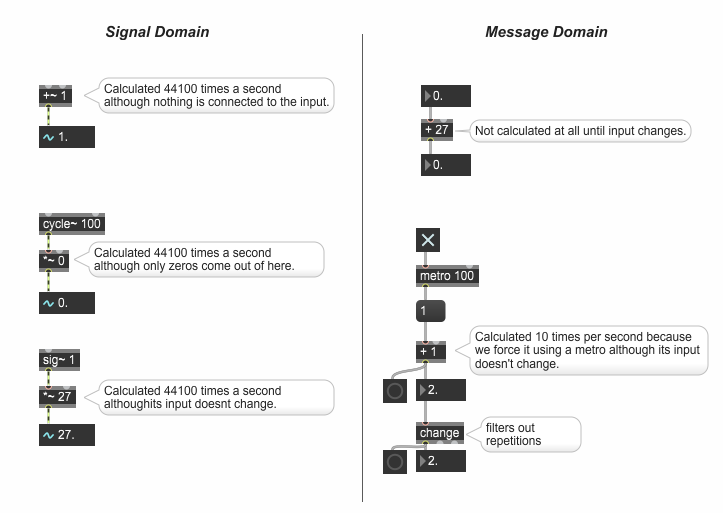
\includegraphics[width=\textwidth]{messageDomainSignalDomain}
	\caption[message domain vs. signal domain]
	{The patcher \href{./patchers/00\_introduction/00\_messageDomainSignalDomain.maxpat}{\texttt{00\_messageDomainSignalDomain.maxpat}} should demonstrate the differences between message domain and signal domain in Max/MSP.}
	\label{fig:mesSig}
\end{figure}

\paragraph{How is this not specific to Max/MSP?} The key points here are not specific to this programming language. If we, for example adjust the volume of a track in pro tools or ableton live or similar, then the information of our fader movement will also be in some kind of message domain.\\
One key aspect here is: some kind of conversion between the two is necessary if we want to switch between them. If we want to control the volume of an audio signal from the message domain we have a problem: we will get noisy output since the message domain is not running at sample rate. Look at a naive attempt to controlling the amplitude of a sine wave:

% Lorem ipsum dolor sit amet, consectetur adipisicing elit, sed do eiusmod
% tempor incididunt ut labore et dolore magna aliqua. Ut enim ad minim veniam,
% quis nostrud exercitation ullamco laboris nisi ut aliquip ex ea commodo
% consequat. Duis aute irure dolor in reprehenderit in voluptate velit esse
% cillum dolore eu fugiat nulla pariatur. Excepteur sint occaecat cupidatat non
% proident, sunt in culpa qui officia deserunt mollit anim id est laborum.


\begin{figure}[H]
	\centering
	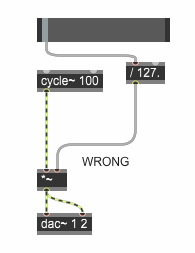
\includegraphics{ampWrong}
	\caption[patcher \texttt{00\_ampWrong.maxpat}]
	{The patcher \href{./patchers/00\_introduction/00\_ampWrong.maxpat}{\texttt{00\_ampWrong.maxpat}}}
	\label{fig:ampWrongRight}
\end{figure}


And let's look at what kind of waveform it will produce:

\begin{figure}[H]
	\centering
	% This file was created with tikzplotlib v0.9.14.
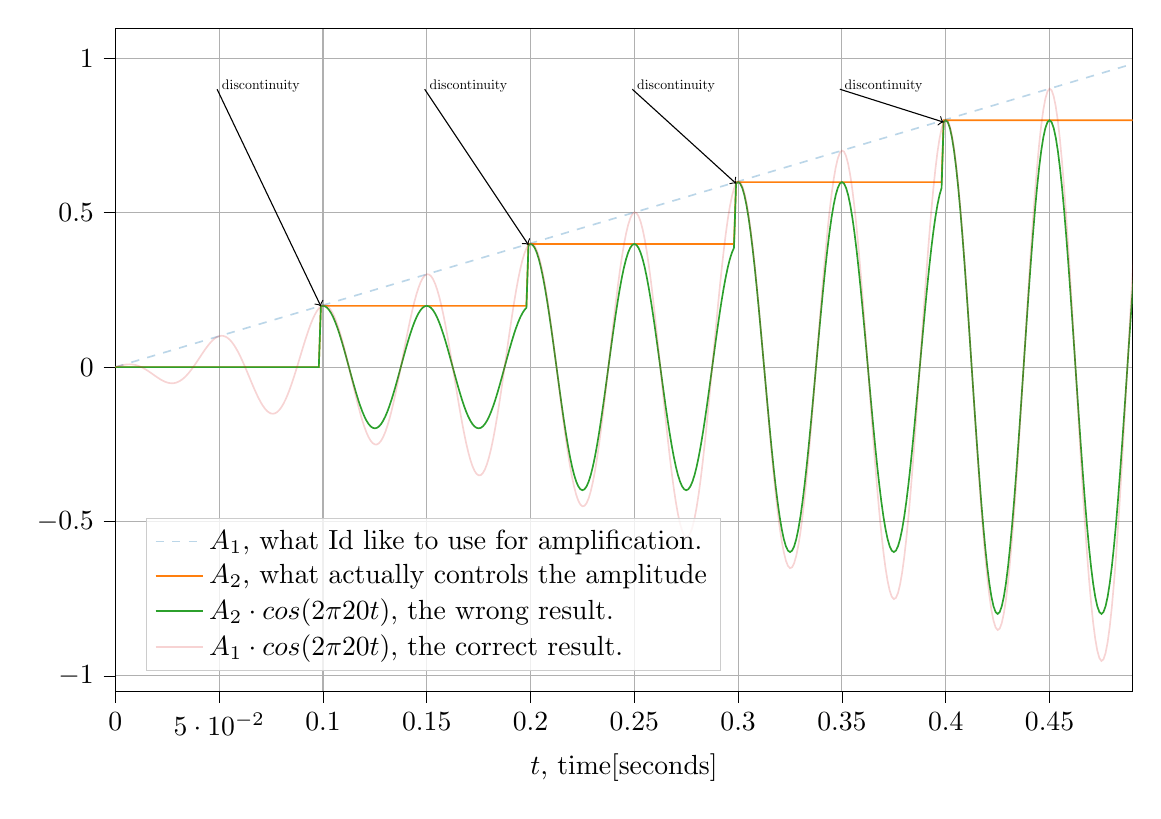
\begin{tikzpicture}

\definecolor{color0}{rgb}{0.12156862745098,0.466666666666667,0.705882352941177}
\definecolor{color1}{rgb}{1,0.498039215686275,0.0549019607843137}
\definecolor{color2}{rgb}{0.172549019607843,0.627450980392157,0.172549019607843}
\definecolor{color3}{rgb}{0.83921568627451,0.152941176470588,0.156862745098039}

\begin{axis}[
height=10cm,
legend cell align={left},
legend style={
  fill opacity=0.8,
  draw opacity=1,
  text opacity=1,
  at={(0.03,0.03)},
  anchor=south west,
  draw=white!80!black
},
tick align=outside,
tick pos=left,
width=14.5cm,
x grid style={white!69.0196078431373!black},
xlabel={\(\displaystyle t\), time[seconds]},
xmajorgrids,
xmin=0, xmax=0.49,
xtick style={color=black},
y grid style={white!69.0196078431373!black},
ymajorgrids,
ymin=-1.04949899799599, ymax=1.09759519038076,
ytick style={color=black}
]
\addplot [semithick, color0, opacity=0.3, dashed]
table {%
0 0
0.001 0.00200400801603206
0.002 0.00400801603206413
0.003 0.00601202404809619
0.004 0.00801603206412826
0.005 0.0100200400801603
0.006 0.0120240480961924
0.007 0.0140280561122244
0.008 0.0160320641282565
0.009 0.0180360721442886
0.01 0.0200400801603206
0.011 0.0220440881763527
0.012 0.0240480961923848
0.013 0.0260521042084168
0.014 0.0280561122244489
0.015 0.030060120240481
0.016 0.032064128256513
0.017 0.0340681362725451
0.018 0.0360721442885771
0.019 0.0380761523046092
0.02 0.0400801603206413
0.021 0.0420841683366733
0.022 0.0440881763527054
0.023 0.0460921843687375
0.024 0.0480961923847695
0.025 0.0501002004008016
0.026 0.0521042084168337
0.027 0.0541082164328657
0.028 0.0561122244488978
0.029 0.0581162324649299
0.03 0.0601202404809619
0.031 0.062124248496994
0.032 0.064128256513026
0.033 0.0661322645290581
0.034 0.0681362725450902
0.035 0.0701402805611222
0.036 0.0721442885771543
0.037 0.0741482965931864
0.038 0.0761523046092184
0.039 0.0781563126252505
0.04 0.0801603206412826
0.041 0.0821643286573146
0.042 0.0841683366733467
0.043 0.0861723446893787
0.044 0.0881763527054108
0.045 0.0901803607214429
0.046 0.0921843687374749
0.047 0.094188376753507
0.048 0.0961923847695391
0.049 0.0981963927855711
0.05 0.100200400801603
0.051 0.102204408817635
0.052 0.104208416833667
0.053 0.106212424849699
0.054 0.108216432865731
0.055 0.110220440881764
0.056 0.112224448897796
0.057 0.114228456913828
0.058 0.11623246492986
0.059 0.118236472945892
0.06 0.120240480961924
0.061 0.122244488977956
0.062 0.124248496993988
0.063 0.12625250501002
0.064 0.128256513026052
0.065 0.130260521042084
0.066 0.132264529058116
0.067 0.134268537074148
0.068 0.13627254509018
0.069 0.138276553106212
0.07 0.140280561122244
0.071 0.142284569138277
0.072 0.144288577154309
0.073 0.146292585170341
0.074 0.148296593186373
0.075 0.150300601202405
0.076 0.152304609218437
0.077 0.154308617234469
0.078 0.156312625250501
0.079 0.158316633266533
0.08 0.160320641282565
0.081 0.162324649298597
0.082 0.164328657314629
0.083 0.166332665330661
0.084 0.168336673346693
0.085 0.170340681362725
0.086 0.172344689378757
0.087 0.17434869739479
0.088 0.176352705410822
0.089 0.178356713426854
0.09 0.180360721442886
0.091 0.182364729458918
0.092 0.18436873747495
0.093 0.186372745490982
0.094 0.188376753507014
0.095 0.190380761523046
0.096 0.192384769539078
0.097 0.19438877755511
0.098 0.196392785571142
0.099 0.198396793587174
0.1 0.200400801603206
0.101 0.202404809619238
0.102 0.204408817635271
0.103 0.206412825651303
0.104 0.208416833667335
0.105 0.210420841683367
0.106 0.212424849699399
0.107 0.214428857715431
0.108 0.216432865731463
0.109 0.218436873747495
0.11 0.220440881763527
0.111 0.222444889779559
0.112 0.224448897795591
0.113 0.226452905811623
0.114 0.228456913827655
0.115 0.230460921843687
0.116 0.232464929859719
0.117 0.234468937875751
0.118 0.236472945891784
0.119 0.238476953907816
0.12 0.240480961923848
0.121 0.24248496993988
0.122 0.244488977955912
0.123 0.246492985971944
0.124 0.248496993987976
0.125 0.250501002004008
0.126 0.25250501002004
0.127 0.254509018036072
0.128 0.256513026052104
0.129 0.258517034068136
0.13 0.260521042084168
0.131 0.2625250501002
0.132 0.264529058116232
0.133 0.266533066132265
0.134 0.268537074148297
0.135 0.270541082164329
0.136 0.272545090180361
0.137 0.274549098196393
0.138 0.276553106212425
0.139 0.278557114228457
0.14 0.280561122244489
0.141 0.282565130260521
0.142 0.284569138276553
0.143 0.286573146292585
0.144 0.288577154308617
0.145 0.290581162324649
0.146 0.292585170340681
0.147 0.294589178356713
0.148 0.296593186372745
0.149 0.298597194388778
0.15 0.30060120240481
0.151 0.302605210420842
0.152 0.304609218436874
0.153 0.306613226452906
0.154 0.308617234468938
0.155 0.31062124248497
0.156 0.312625250501002
0.157 0.314629258517034
0.158 0.316633266533066
0.159 0.318637274549098
0.16 0.32064128256513
0.161 0.322645290581162
0.162 0.324649298597194
0.163 0.326653306613226
0.164 0.328657314629259
0.165 0.330661322645291
0.166 0.332665330661323
0.167 0.334669338677355
0.168 0.336673346693387
0.169 0.338677354709419
0.17 0.340681362725451
0.171 0.342685370741483
0.172 0.344689378757515
0.173 0.346693386773547
0.174 0.348697394789579
0.175 0.350701402805611
0.176 0.352705410821643
0.177 0.354709418837675
0.178 0.356713426853707
0.179 0.358717434869739
0.18 0.360721442885772
0.181 0.362725450901804
0.182 0.364729458917836
0.183 0.366733466933868
0.184 0.3687374749499
0.185 0.370741482965932
0.186 0.372745490981964
0.187 0.374749498997996
0.188 0.376753507014028
0.189 0.37875751503006
0.19 0.380761523046092
0.191 0.382765531062124
0.192 0.384769539078156
0.193 0.386773547094188
0.194 0.38877755511022
0.195 0.390781563126252
0.196 0.392785571142285
0.197 0.394789579158317
0.198 0.396793587174349
0.199 0.398797595190381
0.2 0.400801603206413
0.201 0.402805611222445
0.202 0.404809619238477
0.203 0.406813627254509
0.204 0.408817635270541
0.205 0.410821643286573
0.206 0.412825651302605
0.207 0.414829659318637
0.208 0.416833667334669
0.209 0.418837675350701
0.21 0.420841683366733
0.211 0.422845691382766
0.212 0.424849699398798
0.213 0.42685370741483
0.214 0.428857715430862
0.215 0.430861723446894
0.216 0.432865731462926
0.217 0.434869739478958
0.218 0.43687374749499
0.219 0.438877755511022
0.22 0.440881763527054
0.221 0.442885771543086
0.222 0.444889779559118
0.223 0.44689378757515
0.224 0.448897795591182
0.225 0.450901803607214
0.226 0.452905811623246
0.227 0.454909819639279
0.228 0.456913827655311
0.229 0.458917835671343
0.23 0.460921843687375
0.231 0.462925851703407
0.232 0.464929859719439
0.233 0.466933867735471
0.234 0.468937875751503
0.235 0.470941883767535
0.236 0.472945891783567
0.237 0.474949899799599
0.238 0.476953907815631
0.239 0.478957915831663
0.24 0.480961923847695
0.241 0.482965931863727
0.242 0.48496993987976
0.243 0.486973947895792
0.244 0.488977955911824
0.245 0.490981963927856
0.246 0.492985971943888
0.247 0.49498997995992
0.248 0.496993987975952
0.249 0.498997995991984
0.25 0.501002004008016
0.251 0.503006012024048
0.252 0.50501002004008
0.253 0.507014028056112
0.254 0.509018036072144
0.255 0.511022044088176
0.256 0.513026052104208
0.257 0.51503006012024
0.258 0.517034068136273
0.259 0.519038076152305
0.26 0.521042084168337
0.261 0.523046092184369
0.262 0.525050100200401
0.263 0.527054108216433
0.264 0.529058116232465
0.265 0.531062124248497
0.266 0.533066132264529
0.267 0.535070140280561
0.268 0.537074148296593
0.269 0.539078156312625
0.27 0.541082164328657
0.271 0.543086172344689
0.272 0.545090180360721
0.273 0.547094188376753
0.274 0.549098196392786
0.275 0.551102204408818
0.276 0.55310621242485
0.277 0.555110220440882
0.278 0.557114228456914
0.279 0.559118236472946
0.28 0.561122244488978
0.281 0.56312625250501
0.282 0.565130260521042
0.283 0.567134268537074
0.284 0.569138276553106
0.285 0.571142284569138
0.286 0.57314629258517
0.287 0.575150300601202
0.288 0.577154308617234
0.289 0.579158316633266
0.29 0.581162324649299
0.291 0.583166332665331
0.292 0.585170340681363
0.293 0.587174348697395
0.294 0.589178356713427
0.295 0.591182364729459
0.296 0.593186372745491
0.297 0.595190380761523
0.298 0.597194388777555
0.299 0.599198396793587
0.3 0.601202404809619
0.301 0.603206412825651
0.302 0.605210420841683
0.303 0.607214428857715
0.304 0.609218436873747
0.305 0.61122244488978
0.306 0.613226452905812
0.307 0.615230460921844
0.308 0.617234468937876
0.309 0.619238476953908
0.31 0.62124248496994
0.311 0.623246492985972
0.312 0.625250501002004
0.313 0.627254509018036
0.314 0.629258517034068
0.315 0.6312625250501
0.316 0.633266533066132
0.317 0.635270541082164
0.318 0.637274549098196
0.319 0.639278557114228
0.32 0.64128256513026
0.321 0.643286573146293
0.322 0.645290581162325
0.323 0.647294589178357
0.324 0.649298597194389
0.325 0.651302605210421
0.326 0.653306613226453
0.327 0.655310621242485
0.328 0.657314629258517
0.329 0.659318637274549
0.33 0.661322645290581
0.331 0.663326653306613
0.332 0.665330661322645
0.333 0.667334669338677
0.334 0.669338677354709
0.335 0.671342685370741
0.336 0.673346693386773
0.337 0.675350701402806
0.338 0.677354709418838
0.339 0.67935871743487
0.34 0.681362725450902
0.341 0.683366733466934
0.342 0.685370741482966
0.343 0.687374749498998
0.344 0.68937875751503
0.345 0.691382765531062
0.346 0.693386773547094
0.347 0.695390781563126
0.348 0.697394789579158
0.349 0.69939879759519
0.35 0.701402805611222
0.351 0.703406813627254
0.352 0.705410821643287
0.353 0.707414829659319
0.354 0.709418837675351
0.355 0.711422845691383
0.356 0.713426853707415
0.357 0.715430861723447
0.358 0.717434869739479
0.359 0.719438877755511
0.36 0.721442885771543
0.361 0.723446893787575
0.362 0.725450901803607
0.363 0.727454909819639
0.364 0.729458917835671
0.365 0.731462925851703
0.366 0.733466933867735
0.367 0.735470941883767
0.368 0.7374749498998
0.369 0.739478957915832
0.37 0.741482965931864
0.371 0.743486973947896
0.372 0.745490981963928
0.373 0.74749498997996
0.374 0.749498997995992
0.375 0.751503006012024
0.376 0.753507014028056
0.377 0.755511022044088
0.378 0.75751503006012
0.379 0.759519038076152
0.38 0.761523046092184
0.381 0.763527054108216
0.382 0.765531062124248
0.383 0.767535070140281
0.384 0.769539078156313
0.385 0.771543086172345
0.386 0.773547094188377
0.387 0.775551102204409
0.388 0.777555110220441
0.389 0.779559118236473
0.39 0.781563126252505
0.391 0.783567134268537
0.392 0.785571142284569
0.393 0.787575150300601
0.394 0.789579158316633
0.395 0.791583166332665
0.396 0.793587174348697
0.397 0.795591182364729
0.398 0.797595190380761
0.399 0.799599198396793
0.4 0.801603206412826
0.401 0.803607214428858
0.402 0.80561122244489
0.403 0.807615230460922
0.404 0.809619238476954
0.405 0.811623246492986
0.406 0.813627254509018
0.407 0.81563126252505
0.408 0.817635270541082
0.409 0.819639278557114
0.41 0.821643286573146
0.411 0.823647294589178
0.412 0.82565130260521
0.413 0.827655310621242
0.414 0.829659318637274
0.415 0.831663326653307
0.416 0.833667334669339
0.417 0.835671342685371
0.418 0.837675350701403
0.419 0.839679358717435
0.42 0.841683366733467
0.421 0.843687374749499
0.422 0.845691382765531
0.423 0.847695390781563
0.424 0.849699398797595
0.425 0.851703406813627
0.426 0.853707414829659
0.427 0.855711422845691
0.428 0.857715430861723
0.429 0.859719438877755
0.43 0.861723446893788
0.431 0.86372745490982
0.432 0.865731462925852
0.433 0.867735470941884
0.434 0.869739478957916
0.435 0.871743486973948
0.436 0.87374749498998
0.437 0.875751503006012
0.438 0.877755511022044
0.439 0.879759519038076
0.44 0.881763527054108
0.441 0.88376753507014
0.442 0.885771543086172
0.443 0.887775551102204
0.444 0.889779559118236
0.445 0.891783567134268
0.446 0.8937875751503
0.447 0.895791583166333
0.448 0.897795591182365
0.449 0.899799599198397
0.45 0.901803607214429
0.451 0.903807615230461
0.452 0.905811623246493
0.453 0.907815631262525
0.454 0.909819639278557
0.455 0.911823647294589
0.456 0.913827655310621
0.457 0.915831663326653
0.458 0.917835671342685
0.459 0.919839679358717
0.46 0.921843687374749
0.461 0.923847695390781
0.462 0.925851703406814
0.463 0.927855711422846
0.464 0.929859719438878
0.465 0.93186372745491
0.466 0.933867735470942
0.467 0.935871743486974
0.468 0.937875751503006
0.469 0.939879759519038
0.47 0.94188376753507
0.471 0.943887775551102
0.472 0.945891783567134
0.473 0.947895791583166
0.474 0.949899799599198
0.475 0.95190380761523
0.476 0.953907815631262
0.477 0.955911823647295
0.478 0.957915831663327
0.479 0.959919839679359
0.48 0.961923847695391
0.481 0.963927855711423
0.482 0.965931863727455
0.483 0.967935871743487
0.484 0.969939879759519
0.485 0.971943887775551
0.486 0.973947895791583
0.487 0.975951903807615
0.488 0.977955911823647
0.489 0.979959919839679
0.49 0.981963927855711
0.491 0.983967935871743
0.492 0.985971943887775
0.493 0.987975951903807
0.494 0.98997995991984
0.495 0.991983967935872
0.496 0.993987975951904
0.497 0.995991983967936
0.498 0.997995991983968
0.499 1
};
\addlegendentry{$A_1$, what Id like to use for amplification.}
\addplot [semithick, color1]
table {%
0 0
0.001 0
0.002 0
0.003 0
0.004 0
0.005 0
0.006 0
0.007 0
0.008 0
0.009 0
0.01 0
0.011 0
0.012 0
0.013 0
0.014 0
0.015 0
0.016 0
0.017 0
0.018 0
0.019 0
0.02 0
0.021 0
0.022 0
0.023 0
0.024 0
0.025 0
0.026 0
0.027 0
0.028 0
0.029 0
0.03 0
0.031 0
0.032 0
0.033 0
0.034 0
0.035 0
0.036 0
0.037 0
0.038 0
0.039 0
0.04 0
0.041 0
0.042 0
0.043 0
0.044 0
0.045 0
0.046 0
0.047 0
0.048 0
0.049 0
0.05 0
0.051 0
0.052 0
0.053 0
0.054 0
0.055 0
0.056 0
0.057 0
0.058 0
0.059 0
0.06 0
0.061 0
0.062 0
0.063 0
0.064 0
0.065 0
0.066 0
0.067 0
0.068 0
0.069 0
0.07 0
0.071 0
0.072 0
0.073 0
0.074 0
0.075 0
0.076 0
0.077 0
0.078 0
0.079 0
0.08 0
0.081 0
0.082 0
0.083 0
0.084 0
0.085 0
0.086 0
0.087 0
0.088 0
0.089 0
0.09 0
0.091 0
0.092 0
0.093 0
0.094 0
0.095 0
0.096 0
0.097 0
0.098 0
0.099 0.198396793587174
0.1 0.198396793587174
0.101 0.198396793587174
0.102 0.198396793587174
0.103 0.198396793587174
0.104 0.198396793587174
0.105 0.198396793587174
0.106 0.198396793587174
0.107 0.198396793587174
0.108 0.198396793587174
0.109 0.198396793587174
0.11 0.198396793587174
0.111 0.198396793587174
0.112 0.198396793587174
0.113 0.198396793587174
0.114 0.198396793587174
0.115 0.198396793587174
0.116 0.198396793587174
0.117 0.198396793587174
0.118 0.198396793587174
0.119 0.198396793587174
0.12 0.198396793587174
0.121 0.198396793587174
0.122 0.198396793587174
0.123 0.198396793587174
0.124 0.198396793587174
0.125 0.198396793587174
0.126 0.198396793587174
0.127 0.198396793587174
0.128 0.198396793587174
0.129 0.198396793587174
0.13 0.198396793587174
0.131 0.198396793587174
0.132 0.198396793587174
0.133 0.198396793587174
0.134 0.198396793587174
0.135 0.198396793587174
0.136 0.198396793587174
0.137 0.198396793587174
0.138 0.198396793587174
0.139 0.198396793587174
0.14 0.198396793587174
0.141 0.198396793587174
0.142 0.198396793587174
0.143 0.198396793587174
0.144 0.198396793587174
0.145 0.198396793587174
0.146 0.198396793587174
0.147 0.198396793587174
0.148 0.198396793587174
0.149 0.198396793587174
0.15 0.198396793587174
0.151 0.198396793587174
0.152 0.198396793587174
0.153 0.198396793587174
0.154 0.198396793587174
0.155 0.198396793587174
0.156 0.198396793587174
0.157 0.198396793587174
0.158 0.198396793587174
0.159 0.198396793587174
0.16 0.198396793587174
0.161 0.198396793587174
0.162 0.198396793587174
0.163 0.198396793587174
0.164 0.198396793587174
0.165 0.198396793587174
0.166 0.198396793587174
0.167 0.198396793587174
0.168 0.198396793587174
0.169 0.198396793587174
0.17 0.198396793587174
0.171 0.198396793587174
0.172 0.198396793587174
0.173 0.198396793587174
0.174 0.198396793587174
0.175 0.198396793587174
0.176 0.198396793587174
0.177 0.198396793587174
0.178 0.198396793587174
0.179 0.198396793587174
0.18 0.198396793587174
0.181 0.198396793587174
0.182 0.198396793587174
0.183 0.198396793587174
0.184 0.198396793587174
0.185 0.198396793587174
0.186 0.198396793587174
0.187 0.198396793587174
0.188 0.198396793587174
0.189 0.198396793587174
0.19 0.198396793587174
0.191 0.198396793587174
0.192 0.198396793587174
0.193 0.198396793587174
0.194 0.198396793587174
0.195 0.198396793587174
0.196 0.198396793587174
0.197 0.198396793587174
0.198 0.198396793587174
0.199 0.398797595190381
0.2 0.398797595190381
0.201 0.398797595190381
0.202 0.398797595190381
0.203 0.398797595190381
0.204 0.398797595190381
0.205 0.398797595190381
0.206 0.398797595190381
0.207 0.398797595190381
0.208 0.398797595190381
0.209 0.398797595190381
0.21 0.398797595190381
0.211 0.398797595190381
0.212 0.398797595190381
0.213 0.398797595190381
0.214 0.398797595190381
0.215 0.398797595190381
0.216 0.398797595190381
0.217 0.398797595190381
0.218 0.398797595190381
0.219 0.398797595190381
0.22 0.398797595190381
0.221 0.398797595190381
0.222 0.398797595190381
0.223 0.398797595190381
0.224 0.398797595190381
0.225 0.398797595190381
0.226 0.398797595190381
0.227 0.398797595190381
0.228 0.398797595190381
0.229 0.398797595190381
0.23 0.398797595190381
0.231 0.398797595190381
0.232 0.398797595190381
0.233 0.398797595190381
0.234 0.398797595190381
0.235 0.398797595190381
0.236 0.398797595190381
0.237 0.398797595190381
0.238 0.398797595190381
0.239 0.398797595190381
0.24 0.398797595190381
0.241 0.398797595190381
0.242 0.398797595190381
0.243 0.398797595190381
0.244 0.398797595190381
0.245 0.398797595190381
0.246 0.398797595190381
0.247 0.398797595190381
0.248 0.398797595190381
0.249 0.398797595190381
0.25 0.398797595190381
0.251 0.398797595190381
0.252 0.398797595190381
0.253 0.398797595190381
0.254 0.398797595190381
0.255 0.398797595190381
0.256 0.398797595190381
0.257 0.398797595190381
0.258 0.398797595190381
0.259 0.398797595190381
0.26 0.398797595190381
0.261 0.398797595190381
0.262 0.398797595190381
0.263 0.398797595190381
0.264 0.398797595190381
0.265 0.398797595190381
0.266 0.398797595190381
0.267 0.398797595190381
0.268 0.398797595190381
0.269 0.398797595190381
0.27 0.398797595190381
0.271 0.398797595190381
0.272 0.398797595190381
0.273 0.398797595190381
0.274 0.398797595190381
0.275 0.398797595190381
0.276 0.398797595190381
0.277 0.398797595190381
0.278 0.398797595190381
0.279 0.398797595190381
0.28 0.398797595190381
0.281 0.398797595190381
0.282 0.398797595190381
0.283 0.398797595190381
0.284 0.398797595190381
0.285 0.398797595190381
0.286 0.398797595190381
0.287 0.398797595190381
0.288 0.398797595190381
0.289 0.398797595190381
0.29 0.398797595190381
0.291 0.398797595190381
0.292 0.398797595190381
0.293 0.398797595190381
0.294 0.398797595190381
0.295 0.398797595190381
0.296 0.398797595190381
0.297 0.398797595190381
0.298 0.398797595190381
0.299 0.599198396793587
0.3 0.599198396793587
0.301 0.599198396793587
0.302 0.599198396793587
0.303 0.599198396793587
0.304 0.599198396793587
0.305 0.599198396793587
0.306 0.599198396793587
0.307 0.599198396793587
0.308 0.599198396793587
0.309 0.599198396793587
0.31 0.599198396793587
0.311 0.599198396793587
0.312 0.599198396793587
0.313 0.599198396793587
0.314 0.599198396793587
0.315 0.599198396793587
0.316 0.599198396793587
0.317 0.599198396793587
0.318 0.599198396793587
0.319 0.599198396793587
0.32 0.599198396793587
0.321 0.599198396793587
0.322 0.599198396793587
0.323 0.599198396793587
0.324 0.599198396793587
0.325 0.599198396793587
0.326 0.599198396793587
0.327 0.599198396793587
0.328 0.599198396793587
0.329 0.599198396793587
0.33 0.599198396793587
0.331 0.599198396793587
0.332 0.599198396793587
0.333 0.599198396793587
0.334 0.599198396793587
0.335 0.599198396793587
0.336 0.599198396793587
0.337 0.599198396793587
0.338 0.599198396793587
0.339 0.599198396793587
0.34 0.599198396793587
0.341 0.599198396793587
0.342 0.599198396793587
0.343 0.599198396793587
0.344 0.599198396793587
0.345 0.599198396793587
0.346 0.599198396793587
0.347 0.599198396793587
0.348 0.599198396793587
0.349 0.599198396793587
0.35 0.599198396793587
0.351 0.599198396793587
0.352 0.599198396793587
0.353 0.599198396793587
0.354 0.599198396793587
0.355 0.599198396793587
0.356 0.599198396793587
0.357 0.599198396793587
0.358 0.599198396793587
0.359 0.599198396793587
0.36 0.599198396793587
0.361 0.599198396793587
0.362 0.599198396793587
0.363 0.599198396793587
0.364 0.599198396793587
0.365 0.599198396793587
0.366 0.599198396793587
0.367 0.599198396793587
0.368 0.599198396793587
0.369 0.599198396793587
0.37 0.599198396793587
0.371 0.599198396793587
0.372 0.599198396793587
0.373 0.599198396793587
0.374 0.599198396793587
0.375 0.599198396793587
0.376 0.599198396793587
0.377 0.599198396793587
0.378 0.599198396793587
0.379 0.599198396793587
0.38 0.599198396793587
0.381 0.599198396793587
0.382 0.599198396793587
0.383 0.599198396793587
0.384 0.599198396793587
0.385 0.599198396793587
0.386 0.599198396793587
0.387 0.599198396793587
0.388 0.599198396793587
0.389 0.599198396793587
0.39 0.599198396793587
0.391 0.599198396793587
0.392 0.599198396793587
0.393 0.599198396793587
0.394 0.599198396793587
0.395 0.599198396793587
0.396 0.599198396793587
0.397 0.599198396793587
0.398 0.599198396793587
0.399 0.799599198396793
0.4 0.799599198396793
0.401 0.799599198396793
0.402 0.799599198396793
0.403 0.799599198396793
0.404 0.799599198396793
0.405 0.799599198396793
0.406 0.799599198396793
0.407 0.799599198396793
0.408 0.799599198396793
0.409 0.799599198396793
0.41 0.799599198396793
0.411 0.799599198396793
0.412 0.799599198396793
0.413 0.799599198396793
0.414 0.799599198396793
0.415 0.799599198396793
0.416 0.799599198396793
0.417 0.799599198396793
0.418 0.799599198396793
0.419 0.799599198396793
0.42 0.799599198396793
0.421 0.799599198396793
0.422 0.799599198396793
0.423 0.799599198396793
0.424 0.799599198396793
0.425 0.799599198396793
0.426 0.799599198396793
0.427 0.799599198396793
0.428 0.799599198396793
0.429 0.799599198396793
0.43 0.799599198396793
0.431 0.799599198396793
0.432 0.799599198396793
0.433 0.799599198396793
0.434 0.799599198396793
0.435 0.799599198396793
0.436 0.799599198396793
0.437 0.799599198396793
0.438 0.799599198396793
0.439 0.799599198396793
0.44 0.799599198396793
0.441 0.799599198396793
0.442 0.799599198396793
0.443 0.799599198396793
0.444 0.799599198396793
0.445 0.799599198396793
0.446 0.799599198396793
0.447 0.799599198396793
0.448 0.799599198396793
0.449 0.799599198396793
0.45 0.799599198396793
0.451 0.799599198396793
0.452 0.799599198396793
0.453 0.799599198396793
0.454 0.799599198396793
0.455 0.799599198396793
0.456 0.799599198396793
0.457 0.799599198396793
0.458 0.799599198396793
0.459 0.799599198396793
0.46 0.799599198396793
0.461 0.799599198396793
0.462 0.799599198396793
0.463 0.799599198396793
0.464 0.799599198396793
0.465 0.799599198396793
0.466 0.799599198396793
0.467 0.799599198396793
0.468 0.799599198396793
0.469 0.799599198396793
0.47 0.799599198396793
0.471 0.799599198396793
0.472 0.799599198396793
0.473 0.799599198396793
0.474 0.799599198396793
0.475 0.799599198396793
0.476 0.799599198396793
0.477 0.799599198396793
0.478 0.799599198396793
0.479 0.799599198396793
0.48 0.799599198396793
0.481 0.799599198396793
0.482 0.799599198396793
0.483 0.799599198396793
0.484 0.799599198396793
0.485 0.799599198396793
0.486 0.799599198396793
0.487 0.799599198396793
0.488 0.799599198396793
0.489 0.799599198396793
0.49 0.799599198396793
0.491 0.799599198396793
0.492 0.799599198396793
0.493 0.799599198396793
0.494 0.799599198396793
0.495 0.799599198396793
0.496 0.799599198396793
0.497 0.799599198396793
0.498 0.799599198396793
0.499 0
};
\addlegendentry{$A_2$, what actually controls the amplitude}
\addplot [semithick, color2]
table {%
0 0
0.001 0
0.002 0
0.003 0
0.004 0
0.005 0
0.006 0
0.007 0
0.008 0
0.009 0
0.01 0
0.011 0
0.012 0
0.013 -0
0.014 -0
0.015 -0
0.016 -0
0.017 -0
0.018 -0
0.019 -0
0.02 -0
0.021 -0
0.022 -0
0.023 -0
0.024 -0
0.025 -0
0.026 -0
0.027 -0
0.028 -0
0.029 -0
0.03 -0
0.031 -0
0.032 -0
0.033 -0
0.034 -0
0.035 -0
0.036 -0
0.037 -0
0.038 0
0.039 0
0.04 0
0.041 0
0.042 0
0.043 0
0.044 0
0.045 0
0.046 0
0.047 0
0.048 0
0.049 0
0.05 0
0.051 0
0.052 0
0.053 0
0.054 0
0.055 0
0.056 0
0.057 0
0.058 0
0.059 0
0.06 0
0.061 0
0.062 0
0.063 -0
0.064 -0
0.065 -0
0.066 -0
0.067 -0
0.068 -0
0.069 -0
0.07 -0
0.071 -0
0.072 -0
0.073 -0
0.074 -0
0.075 -0
0.076 -0
0.077 -0
0.078 -0
0.079 -0
0.08 -0
0.081 -0
0.082 -0
0.083 -0
0.084 -0
0.085 -0
0.086 -0
0.087 -0
0.088 0
0.089 0
0.09 0
0.091 0
0.092 0
0.093 0
0.094 0
0.095 0
0.096 0
0.097 0
0.098 0
0.099 0.19683237561149
0.1 0.198396793587174
0.101 0.19683237561149
0.102 0.19216379349045
0.103 0.18446467355298
0.104 0.173856435519725
0.105 0.160506377641523
0.106 0.144625038306052
0.107 0.126462875721684
0.108 0.106306318041925
0.109 0.084473246222329
0.11 0.0613079808479356
0.111 0.0371758519919573
0.112 0.0124574377422887
0.113 -0.0124574377422884
0.114 -0.0371758519919574
0.115 -0.0613079808479354
0.116 -0.0844732462223291
0.117 -0.106306318041925
0.118 -0.126462875721684
0.119 -0.144625038306051
0.12 -0.160506377641523
0.121 -0.173856435519724
0.122 -0.18446467355298
0.123 -0.19216379349045
0.124 -0.19683237561149
0.125 -0.198396793587174
0.126 -0.19683237561149
0.127 -0.19216379349045
0.128 -0.18446467355298
0.129 -0.173856435519724
0.13 -0.160506377641523
0.131 -0.144625038306052
0.132 -0.126462875721684
0.133 -0.106306318041925
0.134 -0.084473246222329
0.135 -0.0613079808479356
0.136 -0.037175851991957
0.137 -0.0124574377422883
0.138 0.0124574377422888
0.139 0.0371758519919574
0.14 0.0613079808479353
0.141 0.0844732462223288
0.142 0.106306318041925
0.143 0.126462875721683
0.144 0.144625038306051
0.145 0.160506377641523
0.146 0.173856435519724
0.147 0.18446467355298
0.148 0.19216379349045
0.149 0.19683237561149
0.15 0.198396793587174
0.151 0.19683237561149
0.152 0.19216379349045
0.153 0.18446467355298
0.154 0.173856435519724
0.155 0.160506377641523
0.156 0.144625038306052
0.157 0.126462875721684
0.158 0.106306318041925
0.159 0.084473246222329
0.16 0.0613079808479356
0.161 0.0371758519919577
0.162 0.0124574377422884
0.163 -0.0124574377422887
0.164 -0.0371758519919574
0.165 -0.0613079808479353
0.166 -0.0844732462223294
0.167 -0.106306318041925
0.168 -0.126462875721684
0.169 -0.144625038306052
0.17 -0.160506377641523
0.171 -0.173856435519725
0.172 -0.18446467355298
0.173 -0.19216379349045
0.174 -0.196832375611489
0.175 -0.198396793587174
0.176 -0.19683237561149
0.177 -0.19216379349045
0.178 -0.18446467355298
0.179 -0.173856435519724
0.18 -0.160506377641523
0.181 -0.144625038306052
0.182 -0.126462875721684
0.183 -0.106306318041926
0.184 -0.0844732462223291
0.185 -0.0613079808479356
0.186 -0.0371758519919577
0.187 -0.0124574377422891
0.188 0.0124574377422887
0.189 0.0371758519919573
0.19 0.0613079808479353
0.191 0.0844732462223287
0.192 0.106306318041925
0.193 0.126462875721684
0.194 0.144625038306052
0.195 0.160506377641523
0.196 0.173856435519724
0.197 0.18446467355298
0.198 0.19216379349045
0.199 0.395652957037237
0.2 0.398797595190381
0.201 0.395652957037236
0.202 0.386268635399995
0.203 0.370792626636798
0.204 0.34946899665076
0.205 0.322634031824879
0.206 0.290710935584892
0.207 0.254203154228436
0.208 0.213686437276194
0.209 0.169799757558016
0.21 0.123235234229689
0.211 0.0747272176403999
0.212 0.0250407081890458
0.213 -0.0250407081890435
0.214 -0.0747272176403991
0.215 -0.123235234229688
0.216 -0.169799757558014
0.217 -0.213686437276192
0.218 -0.254203154228435
0.219 -0.290710935584891
0.22 -0.322634031824879
0.221 -0.349468996650759
0.222 -0.370792626636798
0.223 -0.386268635399995
0.224 -0.395652957037237
0.225 -0.398797595190381
0.226 -0.395652957037237
0.227 -0.386268635399995
0.228 -0.370792626636798
0.229 -0.349468996650759
0.23 -0.322634031824879
0.231 -0.290710935584891
0.232 -0.254203154228435
0.233 -0.213686437276193
0.234 -0.169799757558015
0.235 -0.123235234229689
0.236 -0.0747272176403999
0.237 -0.0250407081890458
0.238 0.0250407081890435
0.239 0.0747272176403976
0.24 0.123235234229688
0.241 0.169799757558014
0.242 0.213686437276192
0.243 0.254203154228434
0.244 0.290710935584891
0.245 0.322634031824878
0.246 0.349468996650759
0.247 0.370792626636797
0.248 0.386268635399995
0.249 0.395652957037237
0.25 0.398797595190381
0.251 0.395652957037237
0.252 0.386268635399995
0.253 0.370792626636798
0.254 0.349468996650759
0.255 0.322634031824878
0.256 0.290710935584891
0.257 0.254203154228435
0.258 0.213686437276193
0.259 0.169799757558015
0.26 0.123235234229689
0.261 0.0747272176404
0.262 0.0250407081890459
0.263 -0.0250407081890463
0.264 -0.0747272176404004
0.265 -0.123235234229689
0.266 -0.169799757558015
0.267 -0.213686437276193
0.268 -0.254203154228435
0.269 -0.290710935584891
0.27 -0.322634031824878
0.271 -0.349468996650759
0.272 -0.370792626636798
0.273 -0.386268635399996
0.274 -0.395652957037237
0.275 -0.398797595190381
0.276 -0.395652957037237
0.277 -0.386268635399995
0.278 -0.370792626636798
0.279 -0.349468996650759
0.28 -0.322634031824879
0.281 -0.29071093558489
0.282 -0.254203154228436
0.283 -0.213686437276194
0.284 -0.169799757558016
0.285 -0.12323523422969
0.286 -0.0747272176404014
0.287 -0.0250407081890473
0.288 0.025040708189042
0.289 0.0747272176403989
0.29 0.123235234229688
0.291 0.169799757558014
0.292 0.213686437276192
0.293 0.254203154228434
0.294 0.29071093558489
0.295 0.322634031824878
0.296 0.349468996650758
0.297 0.370792626636797
0.298 0.386268635399995
0.299 0.594473538462984
0.3 0.599198396793587
0.301 0.594473538462984
0.302 0.580373477309541
0.303 0.557120579720616
0.304 0.525081557781795
0.305 0.484761686008237
0.306 0.436796832863734
0.307 0.381943432735186
0.308 0.321066556510461
0.309 0.255126268893701
0.31 0.185162487611442
0.311 0.112278583288842
0.312 0.0376239786358028
0.313 -0.0376239786357988
0.314 -0.112278583288838
0.315 -0.185162487611443
0.316 -0.255126268893702
0.317 -0.321066556510461
0.318 -0.381943432735187
0.319 -0.436796832863731
0.32 -0.484761686008234
0.321 -0.525081557781793
0.322 -0.557120579720615
0.323 -0.58037347730954
0.324 -0.594473538462984
0.325 -0.599198396793587
0.326 -0.594473538462984
0.327 -0.58037347730954
0.328 -0.557120579720616
0.329 -0.525081557781794
0.33 -0.484761686008236
0.331 -0.436796832863732
0.332 -0.381943432735185
0.333 -0.321066556510459
0.334 -0.255126268893699
0.335 -0.18516248761144
0.336 -0.11227858328884
0.337 -0.0376239786358007
0.338 0.0376239786358009
0.339 0.11227858328884
0.34 0.18516248761144
0.341 0.255126268893703
0.342 0.321066556510463
0.343 0.381943432735188
0.344 0.43679683286373
0.345 0.484761686008233
0.346 0.525081557781792
0.347 0.557120579720614
0.348 0.580373477309539
0.349 0.594473538462983
0.35 0.599198396793587
0.351 0.594473538462984
0.352 0.580373477309541
0.353 0.557120579720616
0.354 0.525081557781795
0.355 0.484761686008237
0.356 0.436796832863734
0.357 0.38194343273519
0.358 0.321066556510461
0.359 0.255126268893701
0.36 0.185162487611442
0.361 0.112278583288842
0.362 0.0376239786358029
0.363 -0.0376239786357987
0.364 -0.112278583288838
0.365 -0.185162487611438
0.366 -0.255126268893698
0.367 -0.321066556510461
0.368 -0.381943432735187
0.369 -0.436796832863731
0.37 -0.484761686008234
0.371 -0.525081557781793
0.372 -0.557120579720615
0.373 -0.58037347730954
0.374 -0.594473538462983
0.375 -0.599198396793587
0.376 -0.594473538462984
0.377 -0.58037347730954
0.378 -0.557120579720616
0.379 -0.525081557781794
0.38 -0.484761686008236
0.381 -0.436796832863733
0.382 -0.381943432735188
0.383 -0.321066556510463
0.384 -0.2551262688937
0.385 -0.18516248761144
0.386 -0.11227858328884
0.387 -0.0376239786358009
0.388 0.0376239786358007
0.389 0.11227858328884
0.39 0.18516248761144
0.391 0.255126268893699
0.392 0.321066556510459
0.393 0.381943432735188
0.394 0.436796832863732
0.395 0.484761686008236
0.396 0.525081557781794
0.397 0.557120579720616
0.398 0.58037347730954
0.399 0.793294119888731
0.4 0.799599198396793
0.401 0.79329411988873
0.402 0.774478319219085
0.403 0.743448532804433
0.404 0.700694118912828
0.405 0.646889340191591
0.406 0.582882730142571
0.407 0.509683711241942
0.408 0.428446675744734
0.409 0.340452780229393
0.41 0.247089740993196
0.411 0.149829948937285
0.412 0.0502072490825599
0.413 -0.0502072490825539
0.414 -0.149829948937279
0.415 -0.24708974099319
0.416 -0.340452780229382
0.417 -0.428446675744724
0.418 -0.509683711241933
0.419 -0.582882730142571
0.42 -0.64688934019159
0.421 -0.700694118912828
0.422 -0.743448532804432
0.423 -0.774478319219085
0.424 -0.79329411988873
0.425 -0.799599198396793
0.426 -0.793294119888731
0.427 -0.774478319219086
0.428 -0.743448532804434
0.429 -0.700694118912829
0.43 -0.646889340191592
0.431 -0.582882730142573
0.432 -0.50968371124194
0.433 -0.428446675744732
0.434 -0.34045278022939
0.435 -0.247089740993199
0.436 -0.149829948937282
0.437 -0.0502072490825572
0.438 0.0502072490825566
0.439 0.149829948937282
0.44 0.247089740993193
0.441 0.340452780229385
0.442 0.428446675744726
0.443 0.509683711241936
0.444 0.582882730142573
0.445 0.646889340191592
0.446 0.700694118912829
0.447 0.743448532804433
0.448 0.774478319219086
0.449 0.793294119888731
0.45 0.799599198396793
0.451 0.793294119888731
0.452 0.774478319219086
0.453 0.743448532804433
0.454 0.700694118912828
0.455 0.646889340191591
0.456 0.582882730142571
0.457 0.509683711241938
0.458 0.428446675744729
0.459 0.340452780229388
0.46 0.247089740993196
0.461 0.149829948937285
0.462 0.0502072490825545
0.463 -0.0502072490825593
0.464 -0.149829948937284
0.465 -0.247089740993195
0.466 -0.340452780229387
0.467 -0.428446675744729
0.468 -0.509683711241938
0.469 -0.582882730142567
0.47 -0.64688934019159
0.471 -0.700694118912828
0.472 -0.743448532804432
0.473 -0.774478319219085
0.474 -0.79329411988873
0.475 -0.799599198396793
0.476 -0.793294119888731
0.477 -0.774478319219087
0.478 -0.743448532804436
0.479 -0.700694118912829
0.48 -0.646889340191592
0.481 -0.582882730142573
0.482 -0.509683711241941
0.483 -0.428446675744732
0.484 -0.340452780229391
0.485 -0.247089740993199
0.486 -0.149829948937288
0.487 -0.050207249082563
0.488 0.0502072490825564
0.489 0.149829948937281
0.49 0.247089740993193
0.491 0.340452780229384
0.492 0.428446675744726
0.493 0.509683711241935
0.494 0.582882730142569
0.495 0.646889340191588
0.496 0.700694118912829
0.497 0.743448532804433
0.498 0.774478319219085
0.499 0
};
\addlegendentry{$A_2 \cdot cos(2\pi 20 t)$, the wrong result.}
\addplot [semithick, color3, opacity=0.2]
table {%
0 0
0.001 0.00198820581425747
0.002 0.00388209683819091
0.003 0.00558983859251454
0.004 0.00702450244524139
0.005 0.00810638270916781
0.006 0.0087651538367304
0.007 0.0089418194954726
0.008 0.00859040953874143
0.009 0.00767938602021173
0.01 0.0061927253381753
0.011 0.0041306502213286
0.012 0.00150999245361074
0.013 -0.0016358251580783
0.014 -0.00525719119078185
0.015 -0.00928908800726295
0.016 -0.0136522418137097
0.017 -0.0182546202698255
0.018 -0.0229932501312152
0.019 -0.0277563204829796
0.02 -0.0324255308366712
0.021 -0.0368786378375173
0.022 -0.0409921496784399
0.023 -0.0446441136391954
0.024 -0.0477169395421793
0.025 -0.0501002004008016
0.026 -0.0516933511706942
0.027 -0.0524083073155772
0.028 -0.052171826863469
0.029 -0.0509276427280001
0.03 -0.0486382962550069
0.031 -0.0452866281564404
0.032 -0.0408768891221604
0.033 -0.0354354393473084
0.034 -0.0290110138541332
0.035 -0.0216745386836136
0.036 -0.0135184916334391
0.037 -0.00465581006529984
0.038 0.00478164276976731
0.039 0.0146450326028923
0.04 0.0247709013527012
0.041 0.0349838696476312
0.042 0.0450996500783925
0.043 0.0549283197579031
0.044 0.0642777948026896
0.045 0.0729574443825103
0.046 0.080781778120276
0.047 0.0875741379493944
0.048 0.0931703241165817
0.049 0.097422084898616
0.05 0.100200400801603
0.051 0.101398496527131
0.052 0.100934517792964
0.053 0.0987538151344235
0.054 0.0948307830107588
0.055 0.0891702098008459
0.056 0.0818081024761504
0.057 0.0728119587488483
0.058 0.0622804691558753
0.059 0.0503426416880547
0.06 0.0371563520290518
0.061 0.0229063330455495
0.062 0.00780162767698883
0.063 -0.00792746038145631
0.064 -0.0240328740150028
0.065 -0.0402527146981394
0.066 -0.0563154974815528
0.067 -0.0719446798869595
0.068 -0.0868633893845911
0.069 -0.1007992691224
0.07 -0.113489357928349
0.071 -0.124684918403035
0.072 -0.134156126220349
0.073 -0.141696534593968
0.074 -0.147127230255053
0.075 -0.150300601202405
0.076 -0.151103641883568
0.077 -0.14946072827035
0.078 -0.145335803405378
0.079 -0.138733923293517
0.08 -0.129702123346685
0.081 -0.11832957679586
0.082 -0.104747028375536
0.083 -0.0891254989644422
0.084 -0.0716742695219761
0.085 -0.0526381653744901
0.086 -0.0322941744576601
0.087 -0.0109474452886782
0.088 0.0110732779931453
0.089 0.0334207154271129
0.09 0.0557345280435776
0.091 0.077647125315474
0.092 0.0987897096955264
0.093 0.118798459011279
0.094 0.13732074344211
0.095 0.154021271474188
0.096 0.168588058685793
0.097 0.180738114491303
0.098 0.190222745071354
0.099 0.19683237561149
0.1 0.200400801603206
0.101 0.200808787240005
0.102 0.197986938747736
0.103 0.191917791676332
0.104 0.182637063576276
0.105 0.170234036892524
0.106 0.154851051115571
0.107 0.136682098002224
0.108 0.115970528773009
0.109 0.0930058973558976
0.11 0.0681199787199284
0.111 0.0416820158697703
0.112 0.014093262900367
0.113 -0.0142190956048343
0.114 -0.0428085568392237
0.115 -0.0712163413890158
0.116 -0.0989787531493957
0.117 -0.125634739504093
0.118 -0.150733528637967
0.119 -0.173842217761819
0.12 -0.194553185020027
0.121 -0.212491198968552
0.122 -0.227320102762258
0.123 -0.238748955548741
0.124 -0.246537520967926
0.125 -0.250501002004008
0.126 -0.250513932596441
0.127 -0.246513149225123
0.128 -0.238499779947287
0.129 -0.226540203859035
0.13 -0.210765950438363
0.131 -0.191372525435281
0.132 -0.168617167628912
0.133 -0.142815558581576
0.134 -0.114337525189819
0.135 -0.0836017920653667
0.136 -0.0510698572818803
0.137 -0.0172390805120556
0.138 0.0173649132165237
0.139 0.0521963982513341
0.14 0.086698154734454
0.141 0.120310380983317
0.142 0.15247976931266
0.143 0.182668598264654
0.144 0.210363692081529
0.145 0.235085098565866
0.146 0.256394339251311
0.147 0.273902091033212
0.148 0.287275166026127
0.149 0.296242666324363
0.15 0.30060120240481
0.151 0.300219077952878
0.152 0.295039359702509
0.153 0.285081768218242
0.154 0.270443344141794
0.155 0.251297863984202
0.156 0.227893999754991
0.157 0.2005522372556
0.158 0.169660588390143
0.159 0.135669153023741
0.16 0.099083605410805
0.161 0.0604576986939918
0.162 0.0203848981237446
0.163 -0.0205107308282128
0.164 -0.0615842396634445
0.165 -0.102179968079892
0.166 -0.141642008817239
0.167 -0.179324799121228
0.168 -0.214603667891343
0.169 -0.24688516640124
0.17 -0.275617012111705
0.171 -0.30029747953407
0.172 -0.320484079304167
0.173 -0.335801376503513
0.174 -0.3459478116808
0.175 -0.350701402805611
0.176 -0.349924223309315
0.177 -0.343565570179895
0.178 -0.331663756489196
0.179 -0.314346484424552
0.18 -0.291829777530041
0.181 -0.264415474074701
0.182 -0.232487306882288
0.183 -0.196505618198711
0.184 -0.157000780857662
0.185 -0.114565418756243
0.186 -0.0698455401061023
0.187 -0.0235307157354349
0.188 0.0236565484399018
0.189 0.0709720810755549
0.19 0.11766178142533
0.191 0.162973636651159
0.192 0.206169828929795
0.193 0.24653873751803
0.194 0.283406640720949
0.195 0.316148925657544
0.196 0.344200619816828
0.197 0.367066067575121
0.198 0.3843275869809
0.199 0.395652957037237
0.2 0.400801603206413
0.201 0.399629368665751
0.202 0.392091780657281
0.203 0.37824574476015
0.204 0.358249624707312
0.205 0.33236169107588
0.206 0.300936948394411
0.207 0.264422376508976
0.208 0.223350648007278
0.209 0.178332408691585
0.21 0.130047232101682
0.211 0.0792333815182129
0.212 0.0266765333471242
0.213 -0.0268023660515893
0.214 -0.0803599224876653
0.215 -0.133143594770768
0.216 -0.184305264485081
0.217 -0.23301485873836
0.218 -0.278473807144718
0.219 -0.319928115040659
0.22 -0.356680839203383
0.221 -0.388103760099586
0.222 -0.413648055846076
0.223 -0.432853797458286
0.224 -0.445358102393673
0.225 -0.450901803607214
0.226 -0.449334514022188
0.227 -0.440617991134668
0.228 -0.424827733031105
0.229 -0.40215276499007
0.23 -0.37289360462172
0.231 -0.33745842271412
0.232 -0.296357446135663
0.233 -0.250195677815844
0.234 -0.199664036525505
0.235 -0.14552904544712
0.236 -0.0886212229303235
0.237 -0.0298223509588134
0.238 0.0299481836632782
0.239 0.089747763899774
0.24 0.148625408116207
0.241 0.205636892319002
0.242 0.259859888546927
0.243 0.310408876771405
0.244 0.356449589360369
0.245 0.397212752749222
0.246 0.432006900382345
0.247 0.46023004411703
0.248 0.481380007935672
0.249 0.49506324775011
0.25 0.501002004008016
0.251 0.499039659378625
0.252 0.489144201612054
0.253 0.471409721302059
0.254 0.446055905272828
0.255 0.413425518167558
0.256 0.37397989703383
0.257 0.328292515762351
0.258 0.277040707624411
0.259 0.220995664359427
0.26 0.161010858792558
0.261 0.0980090643424341
0.262 0.0329681685705026
0.263 -0.0330940012749707
0.264 -0.0991356053118879
0.265 -0.164107221461647
0.266 -0.226968520152925
0.267 -0.286704918355496
0.268 -0.342343946398094
0.269 -0.392971063680079
0.27 -0.437744666295061
0.271 -0.475910040665104
0.272 -0.506812032387986
0.273 -0.529906218413059
0.274 -0.544768393106547
0.275 -0.551102204408818
0.276 -0.548744804735062
0.277 -0.53767041208944
0.278 -0.517991709573014
0.279 -0.489959045555587
0.28 -0.453957431713398
0.281 -0.410501371353538
0.282 -0.36022758538904
0.283 -0.30388573743298
0.284 -0.24232729219335
0.285 -0.176492672137999
0.286 -0.107396905754547
0.287 -0.0361139861821939
0.288 0.0362398188866537
0.289 0.108523446723996
0.29 0.179589034807083
0.291 0.248300147986845
0.292 0.313549948164061
0.293 0.37427901602478
0.294 0.429492537999788
0.295 0.478276579840899
0.296 0.519813180947861
0.297 0.553394020658938
0.298 0.578432428890445
0.299 0.594473538462984
0.3 0.601202404809619
0.301 0.598449950091499
0.302 0.586196622566827
0.303 0.564573697843969
0.304 0.533862185838347
0.305 0.494489345259238
0.306 0.447022845673253
0.307 0.392162655015727
0.308 0.330730767241545
0.309 0.26365892002727
0.31 0.191974485483435
0.311 0.116784747166655
0.312 0.0392598037938811
0.313 -0.0393856364983446
0.314 -0.117911288136105
0.315 -0.195070848152523
0.316 -0.269631775820768
0.317 -0.340394977972629
0.318 -0.40621408565147
0.319 -0.466014012319499
0.32 -0.518808493386739
0.321 -0.563716321230621
0.322 -0.599976008929893
0.323 -0.626958639367831
0.324 -0.644178683819421
0.325 -0.651302605210421
0.326 -0.648155095447935
0.327 -0.634722833044213
0.328 -0.611155686114923
0.329 -0.577765326121105
0.33 -0.535021258805076
0.331 -0.483544319992961
0.332 -0.424097724642413
0.333 -0.35757579705011
0.334 -0.284990547861189
0.335 -0.207456298828871
0.336 -0.126172588578764
0.337 -0.042405621405568
0.338 0.0425314541100357
0.339 0.127299129548217
0.34 0.210552661497959
0.341 0.290963403654692
0.342 0.367240007781198
0.343 0.438149155278159
0.344 0.502535486639207
0.345 0.559340406932577
0.346 0.607619461513378
0.347 0.646557997200846
0.348 0.675484849845216
0.349 0.693883829175856
0.35 0.701402805611222
0.351 0.697860240804372
0.352 0.6832490435216
0.353 0.657737674385878
0.354 0.621668466403865
0.355 0.575553172350917
0.356 0.520065794312673
0.357 0.456032794269106
0.358 0.384420826858679
0.359 0.306322175695113
0.36 0.222938112174312
0.361 0.135560429990877
0.362 0.0455514390172597
0.363 -0.0456772717217221
0.364 -0.136686970960325
0.365 -0.226034474843395
0.366 -0.312295031488606
0.367 -0.394085037589763
0.368 -0.470084224904845
0.369 -0.539056960958919
0.37 -0.599872320478417
0.371 -0.651522601796138
0.372 -0.693139985471802
0.373 -0.724011060322603
0.374 -0.743588974532294
0.375 -0.751503006012024
0.376 -0.747565386160809
0.377 -0.731775253998986
0.378 -0.704319662656832
0.379 -0.665571606686622
0.38 -0.616085085896754
0.381 -0.556587268632382
0.382 -0.487967863895792
0.383 -0.411265856667248
0.384 -0.327653803529032
0.385 -0.238419925519748
0.386 -0.144948271402985
0.387 -0.0486972566289463
0.388 0.0488230893334136
0.389 0.146074812372438
0.39 0.241516288188835
0.391 0.33362665932253
0.392 0.420930067398328
0.393 0.502019294531535
0.394 0.575578435278631
0.395 0.640404234024258
0.396 0.695425742078898
0.397 0.739721973742757
0.398 0.77253727079999
0.399 0.793294119888731
0.4 0.801603206412826
0.401 0.797270531517245
0.402 0.780301464476371
0.403 0.750901650927785
0.404 0.70947474696938
0.405 0.656616999442592
0.406 0.59310874295209
0.407 0.519902933522483
0.408 0.438110886475818
0.409 0.348985431362962
0.41 0.253901738865189
0.411 0.154336112815098
0.412 0.0518430742406383
0.413 -0.0519689069450996
0.414 -0.155462653784545
0.415 -0.25699810153427
0.416 -0.354958287156449
0.417 -0.447775097206892
0.418 -0.533954364158216
0.419 -0.612099909598339
0.42 -0.680936147570095
0.421 -0.739328882361655
0.422 -0.78630396201371
0.423 -0.821063481277376
0.424 -0.842999265245167
0.425 -0.851703406813627
0.426 -0.846975676873683
0.427 -0.828827674953758
0.428 -0.797483639198741
0.429 -0.75337788725214
0.43 -0.697148912988433
0.431 -0.629630217271802
0.432 -0.551838003149169
0.433 -0.464955916284383
0.434 -0.370317059196881
0.435 -0.26938355221063
0.436 -0.163723954227206
0.437 -0.0549888918523245
0.438 0.0551147245567915
0.439 0.164850495196658
0.44 0.272479914879711
0.441 0.376289914990372
0.442 0.474620127015461
0.443 0.565889433784906
0.444 0.648621383918051
0.445 0.721468061115936
0.446 0.783232022644415
0.447 0.832885950284666
0.448 0.869589691754763
0.449 0.892704410601604
0.45 0.901803607214429
0.451 0.896680822230119
0.452 0.877353885431146
0.453 0.844065627469694
0.454 0.797281027534897
0.455 0.73768082653427
0.456 0.66615169159151
0.457 0.583773072775854
0.458 0.491800946092947
0.459 0.3916486870308
0.46 0.284865365556066
0.461 0.173111795639319
0.462 0.0581347094640104
0.463 -0.0582605421684837
0.464 -0.174238336608772
0.465 -0.287961728225152
0.466 -0.397621542824297
0.467 -0.501465156824031
0.468 -0.597824503411596
0.469 -0.685142858237754
0.47 -0.761999974661773
0.471 -0.827135162927172
0.472 -0.879467938555619
0.473 -0.918115902232148
0.474 -0.94240955595804
0.475 -0.95190380761523
0.476 -0.946385967586557
0.477 -0.925880095908533
0.478 -0.890647615740652
0.479 -0.841184167817657
0.48 -0.778212740080111
0.481 -0.702673165911222
0.482 -0.615708142402545
0.483 -0.518645975901517
0.484 -0.412980314864724
0.485 -0.300347178901507
0.486 -0.182499637051434
0.487 -0.0612805270757098
0.488 0.0614063597801692
0.489 0.183626178020879
0.49 0.303443541570587
0.491 0.418953170658215
0.492 0.528310186632595
0.493 0.629759573038281
0.494 0.721664332557466
0.495 0.80253188820761
0.496 0.871038303209933
0.497 0.926049926826575
0.498 0.966642112709535
0.499 0.992114701314478
};
\addlegendentry{$A_1 \cdot cos(2\pi 20 t)$, the correct result.}
\draw[->,draw=black] (axis cs:0.049,0.9) -- (axis cs:0.099,0.19683237561149);
\draw (axis cs:0.049,0.9) node[
  scale=0.5,
  anchor=base west,
  text=black,
  rotate=0.0
]{discontinuity};
\draw[->,draw=black] (axis cs:0.149,0.9) -- (axis cs:0.199,0.395652957037237);
\draw (axis cs:0.149,0.9) node[
  scale=0.5,
  anchor=base west,
  text=black,
  rotate=0.0
]{discontinuity};
\draw[->,draw=black] (axis cs:0.249,0.9) -- (axis cs:0.299,0.594473538462984);
\draw (axis cs:0.249,0.9) node[
  scale=0.5,
  anchor=base west,
  text=black,
  rotate=0.0
]{discontinuity};
\draw[->,draw=black] (axis cs:0.349,0.9) -- (axis cs:0.399,0.793294119888731);
\draw (axis cs:0.349,0.9) node[
  scale=0.5,
  anchor=base west,
  text=black,
  rotate=0.0
]{discontinuity};
\end{axis}

\end{tikzpicture}

	% \includegraphics[width=\textwidth]{ampWrongViz}
	\caption[Amplitude control, message domain ]
	{This is a cosine wave at 20 Hz and the message domain running at 100 millisecond interval to make the effect more extreme and visible}
	\label{fig:msgDomainAmpControl}
\end{figure}


This is a problem, since the sudden jumps produce clicks, crackling or zipper noise (reproduce or open the patcher and hear it for yourself!). These clicks are caused by the fact that the message domain just doesn't produce
the numbers at the rate of the sampling rate. It's too slow, so to speak.\\
In Max/MSP (but also in general) this problem can be solved by interpolation. Max/MSP offers the \pd{line\textasciitilde} object for this situation. It can be used to create signals at sampling rate and we can tell it to ramp to a specified value in a given amount of time. In figure \ref{fig:ampRight} we see it ramping to any value that comes from the \pd{/ 127.} object within 20 milliseconds\footnote{20ms is just an example. It is a reasonable time for this kind of interpolation but really, it is just an example. It could just as well be 50 ms.}. This interpolation reduces the clicks and noise dramatically. Note that the output of \pd{line\textasciitilde} is in the signal domain (thick cable).

\begin{figure}[H]
	\centering
	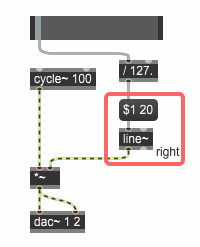
\includegraphics{ampRight}
	\caption[Amplitude control, signal domain]
	{Controlling the amplitude of an oscillator. The interpolation done with \pd{line\textasciitilde} suppresses clicks. }
	\label{fig:ampRight}
\end{figure}


\section{Key Points}
\begin{itemize}
	\item Make sure you understand and know the mathematical notation. It will be how we talk in the remaining chapters.
	\item Make sure you understand what aliasing means in audio.
	\item Make sure you are comfortable with basic mathematical operations on signals, such as adding constants and multiplying with constants
	\item Make sure you understand the difference between message and signal domain and the problem with using a message domain ``signal'' controlling an audio stream.
	\item Make sure you know what the spectrum and time domain signal of an impulse and DC-Offset look like.
\end{itemize}
